\chapter{Occurrence Graph Grammars with NACs}\label{ch:process}

Occurrence Graph Grammars (OGGs) were defined for the Single-Pushout (SPO) approach by~\cite{Ribeiro1996}, and for the Double-Pushout (DPO) approach by~\cite{Corradini1996}. In both cases they consist of a way of representing the concurrent semantics of a graph grammar as a graph grammar itself.

The aim of an OGG is to describe all possible states and changes of states of the graph grammar from which it was constructed. This is possible because occurrence grammars can be regarded as an execution history of the underlying grammar. This history is encoded under the forms of (1) a \emph{core graph} containing all elements ever used in the execution of the grammar and (2) a set of \emph{relations} between the rules and elements of this core graph. 

These relations express dependencies among core graph elements, such as which of them must occur together, at the same state, which ones must be created/deleted one after the other, which elements must never occur together, and so on. They also encode restrictions over the application of rules, such as which rules are sequentially dependent on others or whether it is possible to successfully apply all the rules of a grammar, etc. %This property makes occurrence graph grammars excellent candidates for the generation of test cases, as we are interested in a way of representing several (equivalent) possible derivations using a compact notation.

However, Negative Application Conditions are not addressed by the original definitions of occurrence grammars. Still, NACs are nowadays essential for modelling complex systems as graph grammars, given they provide more compact mechanisms to control the application of rules~\cite{Habel1996, Lambers2008, Corradini2014}. In this chapter, after reviewing the works of~\cite{Ribeiro1996} and~\cite{Corradini1996} in OGGs, and develop an extension of the occurrence grammars framework towards contemplating negative application conditions, which is part of our thesis contribution.

\section{Occurrence Graph Grammars with NACs}

\begin{definition}[Doubly-Typed Graph] Given a type graph $T$, a \emph{doubly-typed graph} \doublyTypedGraph{} over $T$ is a tuple \doublyTypedGraph $= \left(G^T,TG^T, t^{G^T} : G^T \rightarrow TG^T\right)$ where $G^T$ and $TG^T$ are typed graphs over $T$ and \mbox{$t^{G^T} : G^T \rightarrow TG^T$} is a typed graph morphism in \typedGraphCategory{}. We call $TG^T$ the \emph{double-type graph} and $t^{G^T}$ the double-typing morphism.
\end{definition}

\begin{remark}[Typing Morphism] As we are interested in occurrence graph grammars, we will consider only doubly-typed graphs whose typing morphism $type_{TG} : TG \rightarrow T$ is an epimorphism. This has the effect that every element present in $T$ is the image of at least one element from $TG$.
\end{remark}

\begin{example}[Doubly-Typed Graph Example] Figure~\ref{fig:process:doubly-typed-graph} shows a doubly-typed graph $G^{TG^T}$.
\end{example}

\begin{figure}[!ht]
  \centering
  \fbox{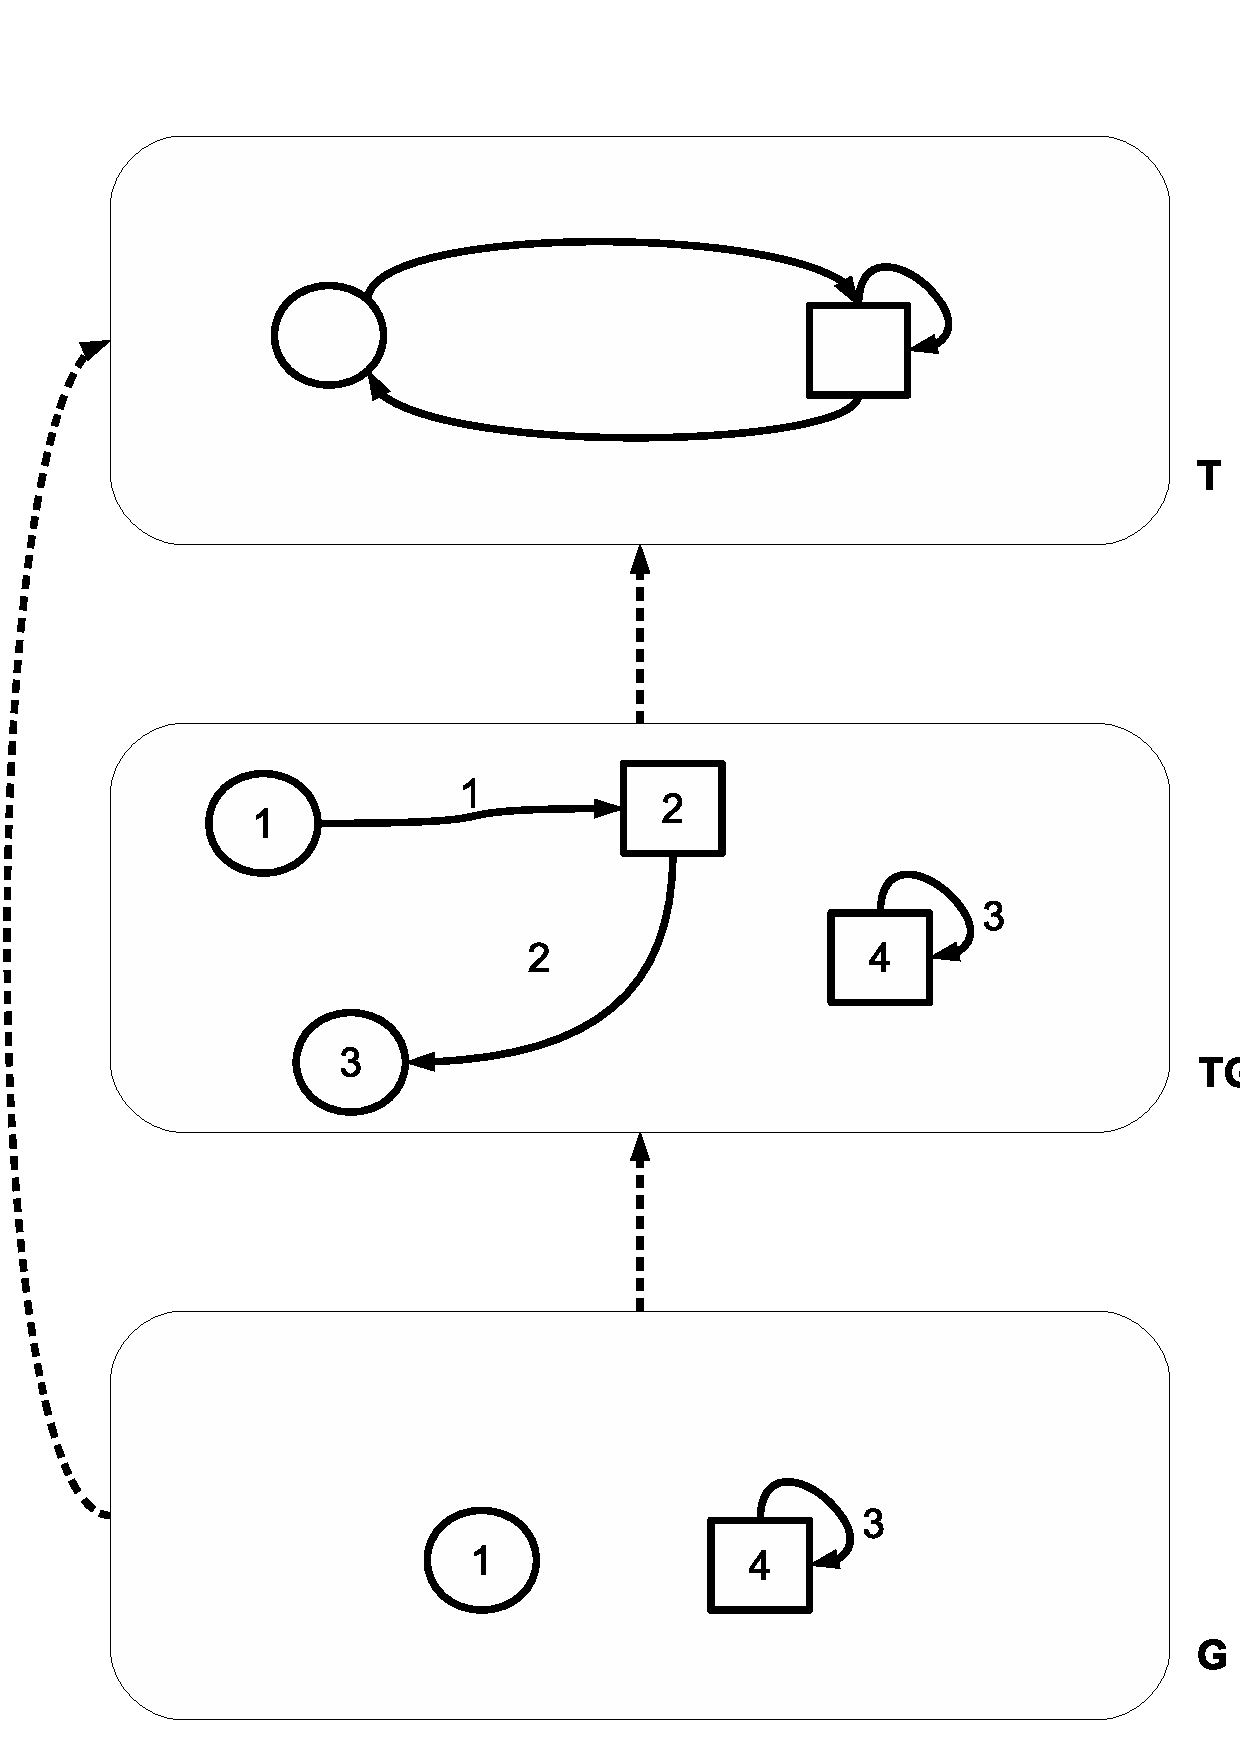
\includegraphics[scale=0.6]{images/process/doubly-typed-graph-example}}
  \caption{Doubly-typed graph}\label{fig:process:doubly-typed-graph}
\end{figure}

\begin{definition}[Doubly-Typed Graph Morphism]
  Given two doubly-typed graphs $G^{TG^T}$ and $H^{TG^T}$ and a graph morphism $g^T : G^T \rightarrow H^T$, we say that $g^T$ is a \emph{$TG^T$-doubly-typed graph morphism} if the following diagram commutes:

\diagram{
  G\ar[rr]^{g}\ar[dr]_{t^{G}}& & H\ar[dl]^{t^{H}} \\
   & TG\ar[d]^{type_{TG}} & \\
  & T &
}
\end{definition}

Notice that the (single) type morphisms $type_G : G \rightarrow T$ and $type_H : H \rightarrow T$ can be obtained respectively as $type_{TG} \circ t^G$ and $type_{TG} \circ t^H$.

\begin{example}[Doubly-Typed Graph Morphism Example] Figure~\ref{fig:process:doubly-typed-graph-morphism} shows a doubly-typed graph morphism $f : G^{TG^T} \rightarrow H^{TG^T}$.
\end{example}

\begin{figure}[!ht]
  \centering
  \fbox{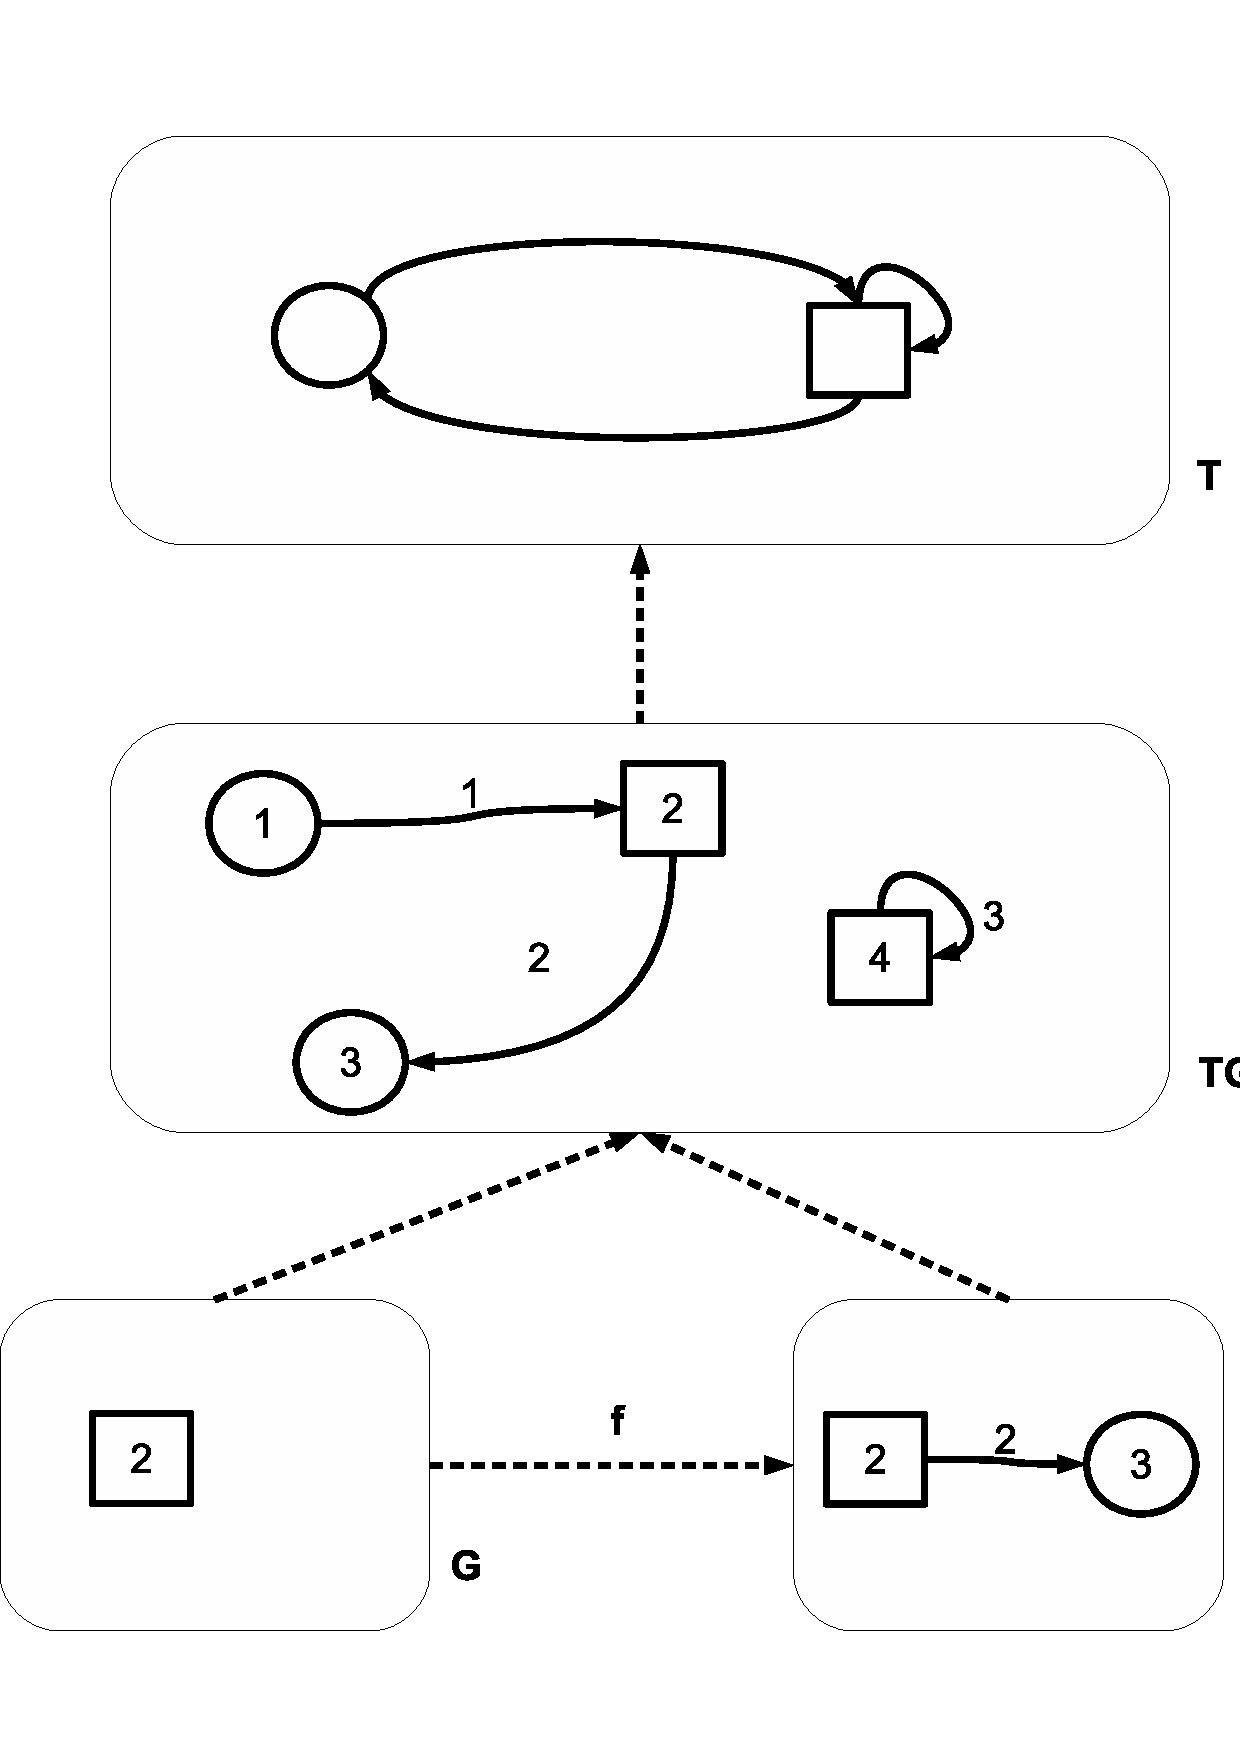
\includegraphics[scale=0.6]{images/process/doubly-typed-graph-morphism-example}}
  \caption{Doubly-typed graph morphism}\label{fig:process:doubly-typed-graph-morphism}
\end{figure}

\begin{remark} \cite{Ribeiro1996} defined different kinds of doubly-typed graph morphisms based on whether the double-type graphs and the type graphs are or are not the same. In this work we are only interested in the case where all doubly-typed graphs share exactly the same double-type and type graphs. Therefore, through the rest of this thesis, we will refer to \mbox{\emph{$TG^T$-doubly-typed graph morphisms}} simply by \emph{doubly-typed graph morphisms}.
\end{remark}


\begin{definition}[Doubly-Typed Graph Rule] A doubly-typed graph rule \doublyTypedRule{} is a span of injective doubly-typed graph morphisms $l : K \rightarrow L$ and $r : K \rightarrow R$.

\diagram{
  L\ar[dr] & K\ar[l]\ar[r]\ar[d] & R\ar[dl]\\
    & TG\ar[d] & \\
    & T &
}

  Given a doubly-typed graph rule \doublyTypedRule{}, its inverse rule is defined by \inverseDoublyTypedRule{}.

  Let the double-typing morphisms from $L^{TG^T}$, $K^{TG^T}$ and $R^{TG^T}$ be $t^{L^T}$, $t^{K^T}$ and $t^{R^T}$, respectively. For a rule $a = p^{TG^T}$ we call:

  \begin{itemize}
    \item $L_a = L_T$, $K_a = K_R$ and $R_a = R_T$, the left, gluing and right graphs of $a$.
    \item $pre_a = t^{L^T} : L^T \rightarrow TG^T$, the \emph{pre-condition} of the $a$.
    \item $post_a = t^{R^T} : R^T \rightarrow TG^T$, the \emph{post-condition} of $a$.
    %\item $r_a = r^T$, the \emph{rule pattern} of $a$.\tinytodo{Not sure if we will need the rule pattern.}
  \end{itemize}
\end{definition}

\begin{example}[Doubly-Typed Graph Rule Example]Figure~\ref{fig:process:doubly-typed-graph-rule} shows a doubly-typed graph rule which deletes an edge $\curvearrowleft_1$ and a node $\Circle_1$, preserves a $\Square_2$ and creates a node $\Circle_3$ and an edge $\curvearrowleft_2$.
\end{example}

\begin{figure}[!ht]
  \centering
  \fbox{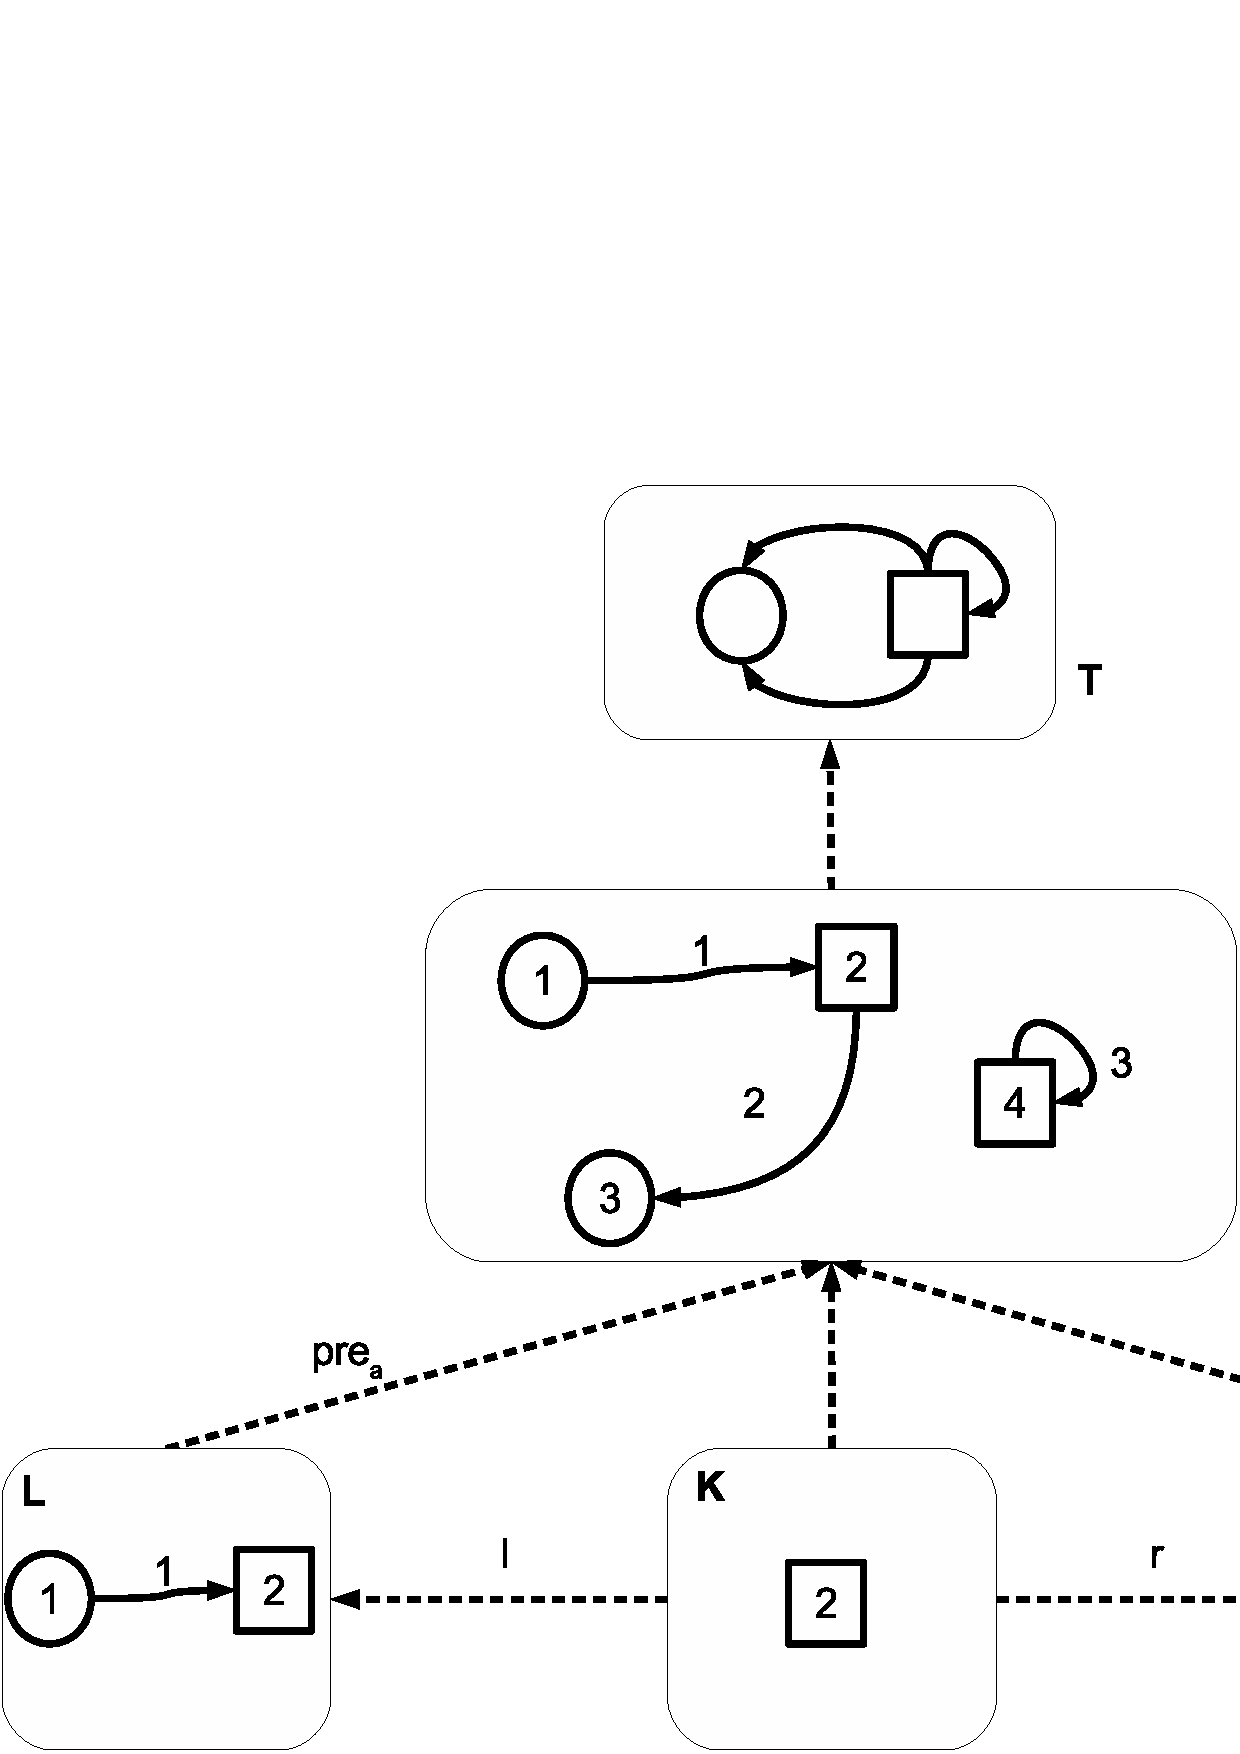
\includegraphics[scale=0.5]{images/process/doubly-typed-graph-rule-example}}
  \caption{Doubly-typed graph rule}\label{fig:process:doubly-typed-graph-rule}
\end{figure}

\begin{definition}[Negative Application Conditions on Doubly-Typed Graph Rules] A \emph{left} negative application condition over a doubly-typed graph rule $p^{TG^T}$ is of the form $NAC(n^T)$, where $n^T : L^T \rightarrow N^T$ is an arbitrary (single-)typed graph morphism. 
 
A (doubly-typed) match morphism $m^{TG^T} : L^{TG^T} \rightarrow G^{TG^T}$ of a rule $p^{TG^T}$ satisfies $NAC(n^T)$ on $L^{TG^T}$, written \mbox{$m^T \models NAC(n^T)$}, iff $\nexists$ $q^T : N^T \rightarrow G^T$ where $q^T$ injective and $q^T \circ n^T = m^T$.

\diagram{
  T & TG\ar[l]\\
  N\ar[u]\ar@{.>}[dr]|{|}_{q} & L\ar[u]\ar[d]^{m}\ar[l]_{n}\\
   & G\ar@/_2.1pc/[uu]
}

  A match $m^{TG^T} : L^{TG^T} \rightarrow G^{TG^T}$ satisfies a set \mbox{$NAC_L = \{NAC\left(n^T_i\right)|i \in I\}$} of left $NACs$, iff \mbox{$m \models NAC\left(n^T_i\right)$} $\forall i \in I$.

\emph{Right} negative application conditions are defined analogously for the right hand side of a rule and its comatch.
\end{definition}

\begin{remark}
  We could have defined NACs whose morphisms are doubly-typed graph morphisms, which would then act specifically over doubly-typed graphs. However, the use of this kind of NAC could lead to a doubly-typed grammar with a set of NACs much bigger than the original one, thus we will not use this kind of NACs given our interest in a compact and more abstract characterization for the semantics of graph grammars. Therefore, we will use \emph{single-typed} NACs as the only NAC type in all of our \emph{doubly-typed graph grammars}, and $NAC(n)$ as a synonym of $NAC(n^T)$.
\end{remark}

In a grammar without NACs, if there is a sequence of graph transformations $t_0\ldots t_n$ where each pair $(t_i,t_{i+1})$ of consecutive transformations is sequentially independent, then it is possible to \emph{switch} the
order of application for any pair in that sequence an arbitrary number of times and still achieve the same final graph as a result (up to isomorphism). This property is called \emph{switch equivalence}~\cite{Corradini2013}.

However, the switch equivalence does not always hold when the grammar has NACs. This happens because there may be situations where the NAC of a rule can be triggered by the cumulative effect of applying two (or more) other rules, while the same rules would not trigger that NAC in isolation. This may lead to a situation where conflicts and dependencies
	are not \emph{stable under switch}, which means that conflicts or dependencies that do not occur in a given sequence of transformations may arise if one or more pairs of transformations are switched. An example is shown in Figure~\ref{ex:process:instability}.

\begin{example}[Switch Equivalence]\label{ex:process:instability}The rules depicted in Figure~\ref{fig:process:instability} show a situation where the independence between rules is not stable under switch equivalence.

  In this example, all rules are independent and also do not conflict with each other in the sense of Definitions~\ref{def:classic-dependency} and~\ref{def:classic-conflict}. 
  Thus, in theory, it should be possible to apply these rules in any order or in parallel. Particularly, it may be possible to apply all rules in the order they appear in the figure: $[p_1, p_2, p_3]$. 
  It may also be possible to apply them in the orders $[p_1, p_3, p_2]$, $[p_2, p_1, p_3]$ and $[p_3, p_1, p_2]$. 
  However, it is not possible to perform a derivation using the rules in the orders $[p_2, p_3, p_1]$ or $[p_3, p_2, p_1]$. This problem arises from the fact that $p_2$ and $p_3$ independently create a piece of the pattern forbidden by the NAC of $p_1$ in a way that, although the effect of each rule by itself does not trigger the NAC of $p_1$, their combined effects do.
\end{example}

\begin{figure}[!ht]
  \centering
  \fbox{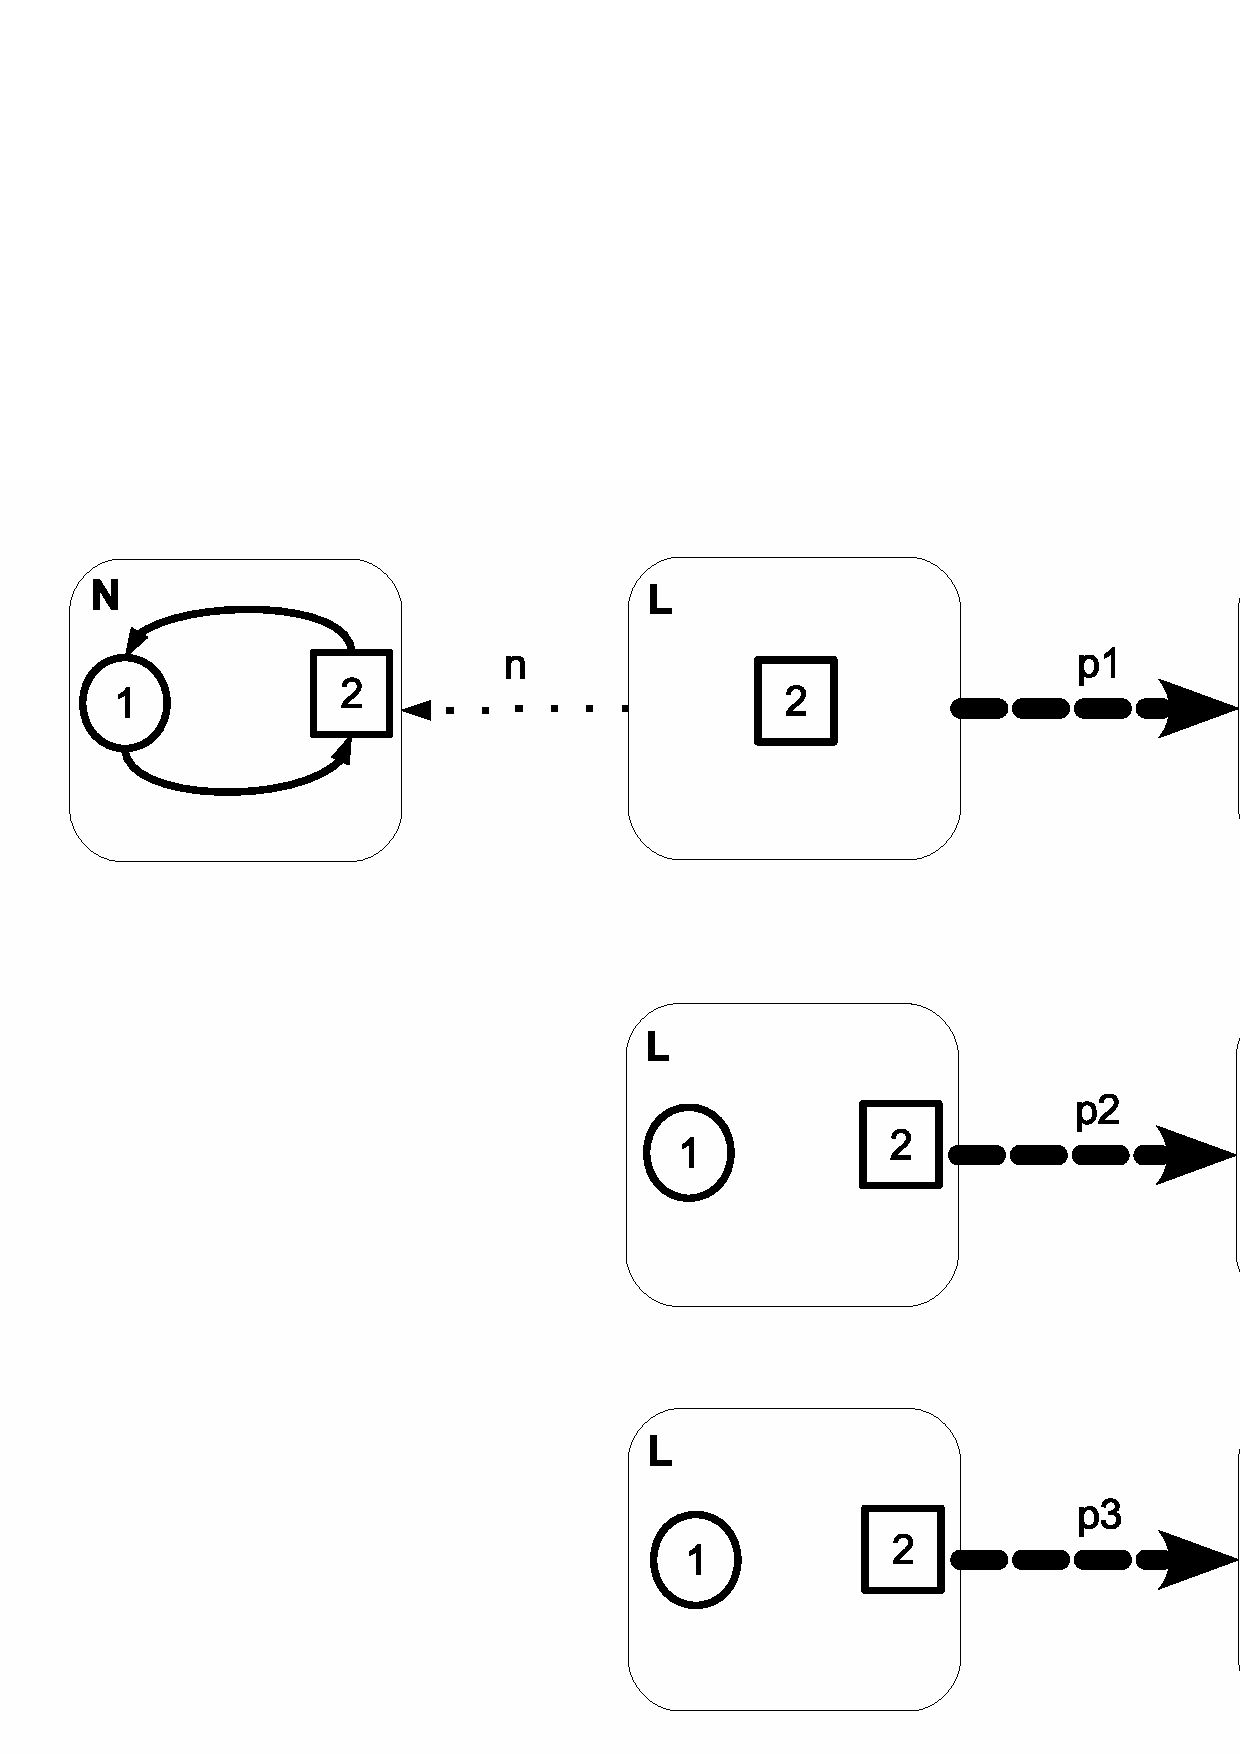
\includegraphics[scale=0.5]{images/process/instability-example}}
  \caption{Instability of conflicts under shift\\}\label{fig:process:instability}
\end{figure}

In order to avoid this problem while we construct a canonical representation of several possible derivations for a set of rules, we will restrict the use of NACs to a special type of NACs called \emph{incremental NACs}.
\emph{Incremental NACs} were originally defined in~\cite{Corradini2013} and~\cite{Corradini2014}. They have the property of extending the forbidden context of a match by a single edge or a single node. Thus, each NAC forbids only one element at a time and therefore there is no possible way to trigger a NAC by the cumulative effects of more than one rule.

\begin{definition}[Incremental NACs] Given a monomorphism \mbox{$n : L \rightarrow N$}, $NAC(n)$ is said to be incremental if for any possible pair of decompositions \mbox{$g_1 : L \rightarrow O_g;g_2 : O_g \rightarrow N$} and \mbox{$f_1 : L \rightarrow O_f;f_2 : O_f \rightarrow N$} as in the diagram below, where all morphisms are monos and \mbox{$f_1;f_2 = n = g_1;g_2$}, there exists a mediating morphism $o_1 : O_g \rightarrow O_f$ or $o_2 : O_f \rightarrow O_g$, such that the resulting triangles
  commutes.

\diagram{
  & O_g\ar[dr]^{g_2}\ar@{.>}@/_0.5pc/[dd]|<<<<<<{o_1} &  \\
  L\ar[ur]^{g_1}\ar[dr]_{f_1}\ar[rr]|<<<<{n}&     & N\\
    & O_f\ar[ur]_{f_2}\ar@{.>}@/_0.5pc/[uu]|<<<<<<<<{o_2} & 
}

\end{definition}

\begin{example}[Incremental NACs]Figure~\ref{fig:process:incremental-nacs} shows all possible (canonical) formats that any valid incremental NAC may assume.

\begin{figure}[!ht]
  \centering
  \fbox{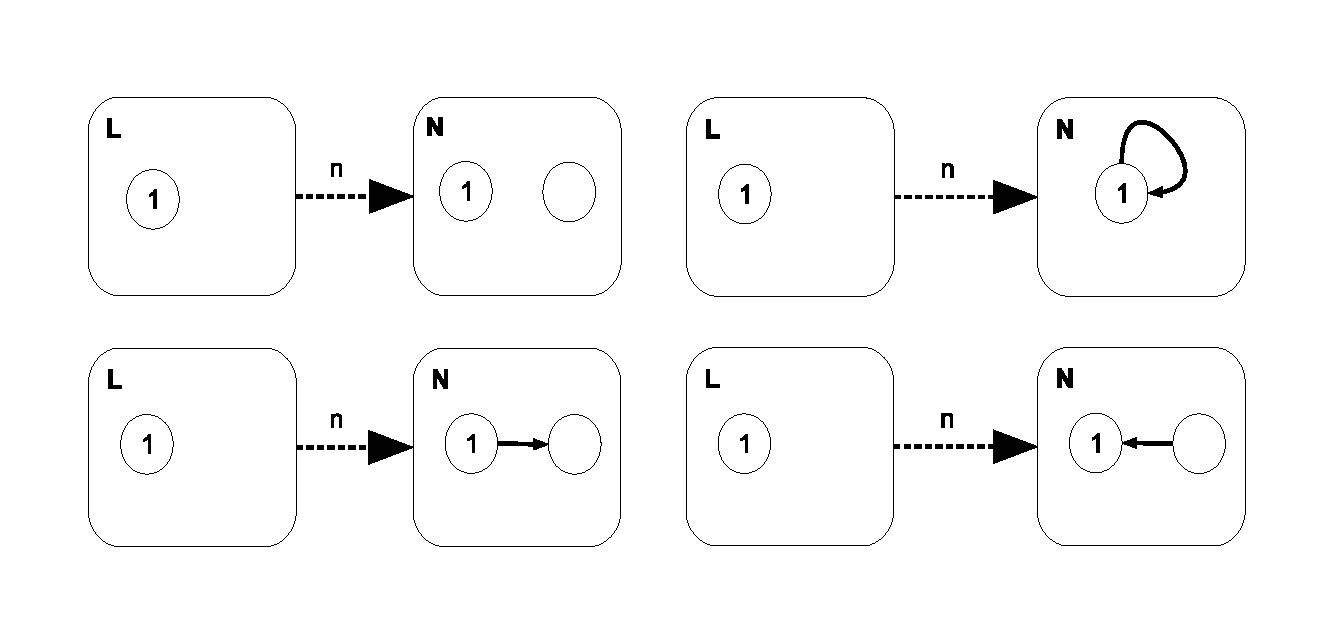
\includegraphics[scale=0.7]{images/process/incremental-nacs}}
  \caption{Canonical Incremental NACs}\label{fig:process:incremental-nacs}
\end{figure}
\end{example}

At first, it may seem that we are loosing expressive power by restricting the NACs used in our grammars to incremental NACs only. However ~\cite{Corradini2013} have shown two important results regarding them. First, they showed that incremental NACs are sufficient to model most of real applications using $GTS$s. Second, they presented an algorithm to compile rules with general NACs to rules with incremental NACs only, generating a new $GTS$ that is able to simulate the original one.

  \begin{notation}[Set Operations over Graphs] Given a graph $G$, we will sometimes view them as being composed of a set $V(G)$ of nodes and a set $E(G)$ of edges, denoted \mbox{$G = V(G) \cup E(G)$}, in order to allow the use of set operations over this graph.
    For example, we say that an element (a node or an edge) $x$ is a member of $G$, denoted $x \in G$, iff $x \in V(G) \cup E(G)$. 
      Moreover, any operations involving multiple graphs will be applied \emph{setwise}. For example, given two graphs $G_1$ and $G_2$, the difference $D = G_1 - G_2$ between them is the union of the differences between their sets of nodes and their sets of edges. Therefore $D = V(D) \cup E(D)$ where $V(D) = V(G_1) - V(G_2)$ and $E(D) = E(G_1) - E(G_2)$.

    Any other set operations applied over graphs will be regarded likewise.
%\mbox{$D = G_1 - G_2 = V(G_1) \cup E(G_1) - V(G_2) \cup E(V_2) = (V(G_1) - V(G_2)) \cup (E(G_1) - E(G_2))$}

\end{notation}

\begin{definition}[Triggering element] Given a rule \graphrule{} with an incremental, non trivially triggered NAC \nac{}, and a monomorphic match \match{}, where there is an injective $q : N \rightarrow G$, therefore $m \not\models NAC(n)$. There is exactly one element that will complete the match towards triggering the NAC, this element is present in the difference between the images of $q$ and $m$.

  Let $G_{|N}$ be the image of $q$, $G_{|L}$ the image of $m$, and \mbox{$D = G_{|N} - G_{|L}$}. The triggering element of this NAC is:

  \begin{itemize}
    \item $x \in E(D)$, if $E(D) \neq \varnothing$;
    \item $x \in V(D)$ otherwise.
  \end{itemize} 
\end{definition}

\begin{example}[Triggering Element]
  Given that incremental NACs extend the match by forbidding only one element at a time, this element can be easily identified at the instance graph: it corresponds to the solely element mapped by the morphism \morph{q}{N}{G} which is not also mapped by \morph{m}{L}{G}. Figure~\ref{fig:process:triggering-element} shows an example. The elements in the instance graph mapped by either $q$ or $m$ are represented by dashed lines. Notice that the only element which is not in the image of
  both morphisms is $\curvearrowleft_2$, therefore $\curvearrowleft_2$ is the triggering element of the NAC for this match.
\end{example}

\begin{figure}[!ht]
  \centering
  \fbox{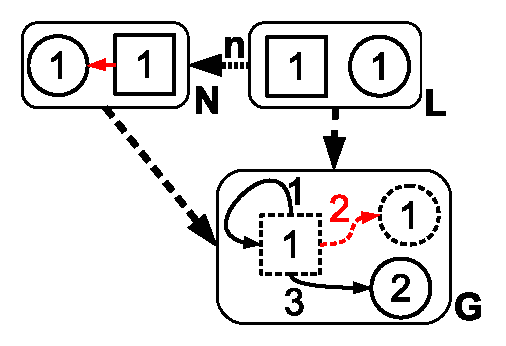
\includegraphics[scale=0.7]{images/process/triggering-element}}
  \caption{Triggering Element}\label{fig:process:triggering-element}
\end{figure}

\begin{definition}[Doubly-Typed Graph Grammars] A \emph{doubly-typed graph grammar} is a tuple $GG = \left(TG^T, I^{TG^T},P \right)$ where $TG^T$ is the double-type graph of the grammar, $I^{TG^T}$ is a doubly-typed graph called the \emph{initial graph} and $P$ is a set of doubly-typed graph rules.

\end{definition}


\begin{definition}[Core Graph]\label{def:core-graph} Given a doubly-typed graph grammar \doublyTypedGraphGrammarCore{}, we have that \coreGraph{} is a \emph{core graph} iff the following two conditions hold:

\begin{description}

  \item[(uniqueness of origin)] \mbox{$\forall x \in$ \coreGraph $: \exists! y \in (I^T \uplus (\uplus_{i \in P} (R_i - K_i))$}:
\[ x =
    \begin{cases}
      in_{GG}\parens{y},$ if $y \in I^T\\
      post_i(y),$ if $y \in R_i - K_i\\
    \end{cases}
   \]

 \item[(uniqueness of deletion)] \mbox{$\forall x \in$ \coreGraph $: \exists^{\leq1} y \in \uplus_{i \in P} (L_i - K_i)$}:
\[ x =
    \begin{cases}
      pre_i(y),$ if $y \in L_i - K_i\\
    \end{cases}
   \]\end{description}

\end{definition}
  The first condition assures that every element in the \emph{core graph} was either already present in the initial graph or was created by one and only one rule. The second condition assures that for every element that is deleted, it is deleted only once by only one rule. The idea is that each element within a \emph{core graph} has a unique origin. At the same time, the \emph{core graph} contains all elements necessary (created, deleted and preserved) by all rules in its underlying grammar. 
  
  In~\cite{Ribeiro1996} the second condition was not used, because of a peculiarity of the SPO approach where more than one rule can delete the same element at the same time, while this would raise a conflict and therefore be forbidden in the DPO approach. As a consequence, the occurrence grammars defined by~\cite{Ribeiro1996} are inherently non-deterministic, whereas ours are deterministic.  In practice, this means that the semantics of a graph grammar in the SPO approach can be achieved with only one occurrence grammar, while in the DPO approach we will need a set of them.

\begin{example}[Doubly-Typed Graph Grammar and Core Graph Example] \mbox{Figure~\ref{fig:process:core-graph:counter-example}} shows a doubly-typed graph grammar, whose double-type is not a core graph. That happens because $\Square_2$ is created by both rules $p_1$ and $p_2$, as well as $\Circle_1$ is deleted by both $p_2$ and $p_3$.

  On the other hand, Figure~\ref{fig:process:core-graph:example} shows a doubly-typed graph grammar whose double-type is also a core graph: $\Square_2$ and $\curvearrowleft_1$ are created by $p_1$, $\curvearrowleft_3$ by $p_2$, $\Circle_3$ and $\curvearrowleft_2$ by $p_3$ and $\Circle_1$ is present on the initial graph. Also, the deleted elements are deleted only once: $\Circle_1$ and
  $\curvearrowleft_1$ by $p_3$.

  It is important to notice that, even though the $TG$ graphs in both grammars are isomorphic, only the one in Figure~\ref{fig:process:core-graph:example} is a core graph. This can be explained by looking to their underlying grammars (initial graphs and rules), where one of them satisfies the conditions presented in Definition~\ref{def:core-graph} while the other does not.
\begin{figure}[!ht]
  \centering
  \begin{subfigure}[t]{.5\textwidth}
    \centerline{\fbox{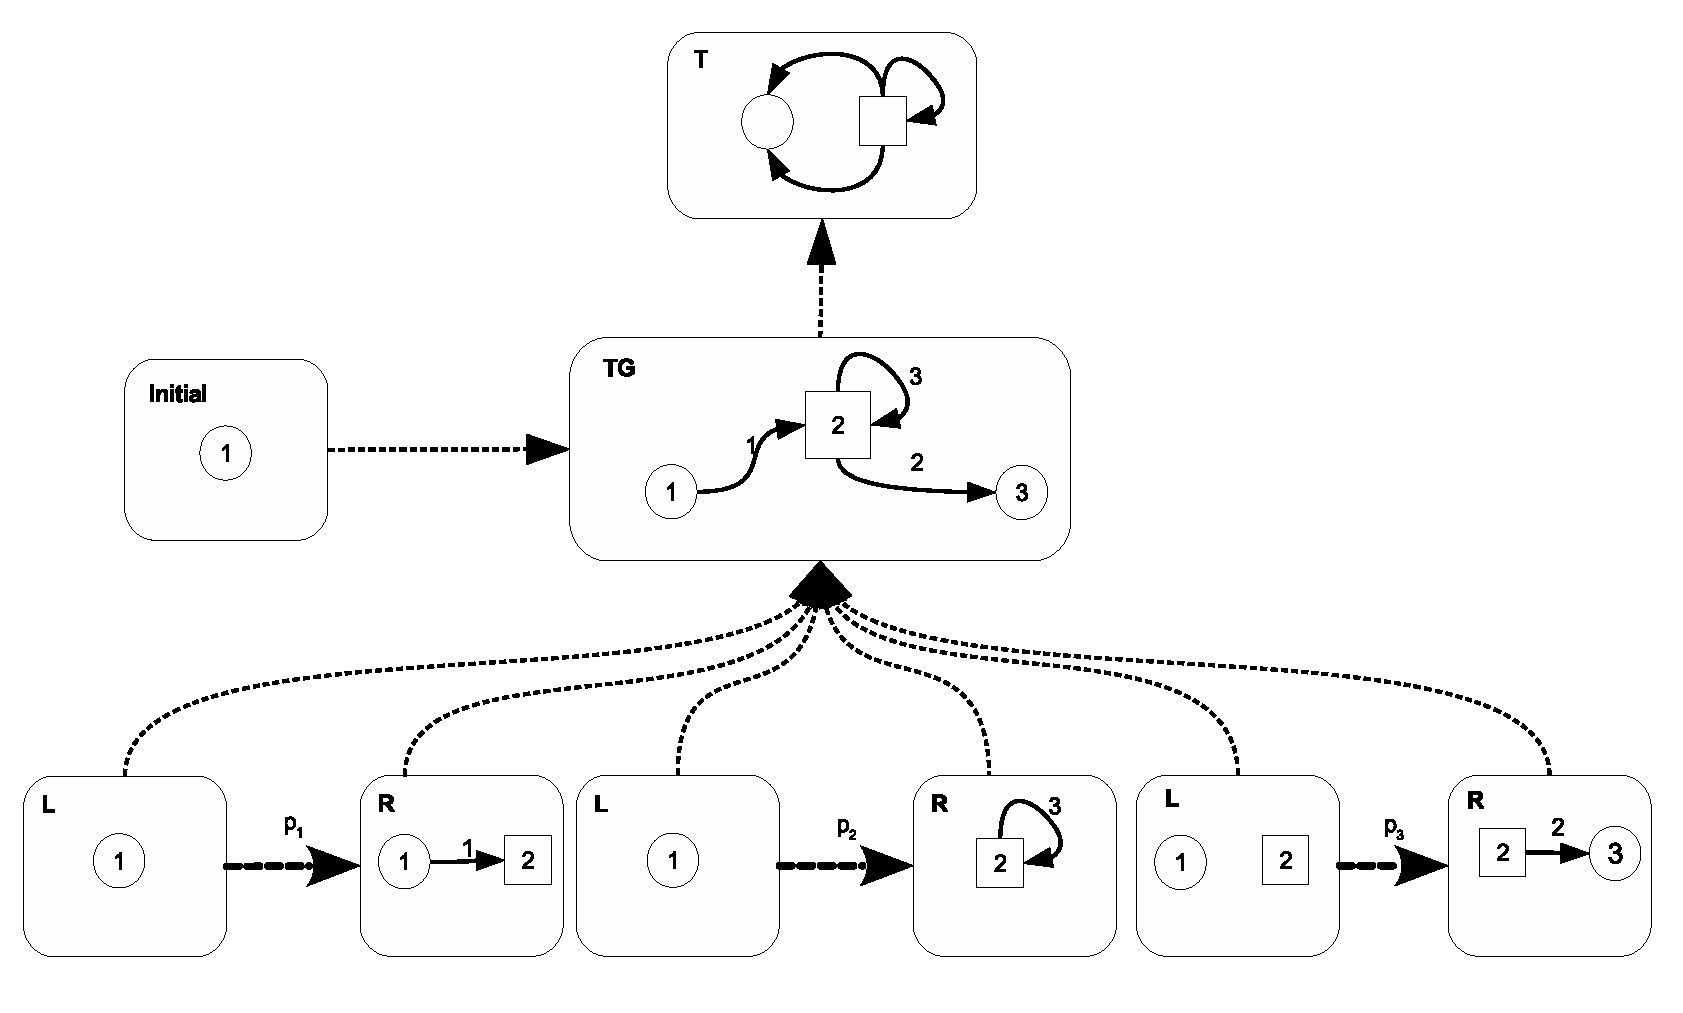
\includegraphics[scale=0.5]{images/process/core_graph/counter_example}}}
    \caption{A grammar with a double-type graph that is not a core graph.}\label{fig:process:core-graph:counter-example}
  \end{subfigure}
  \begin{subfigure}[t]{.5\textwidth}
    \centerline{\fbox{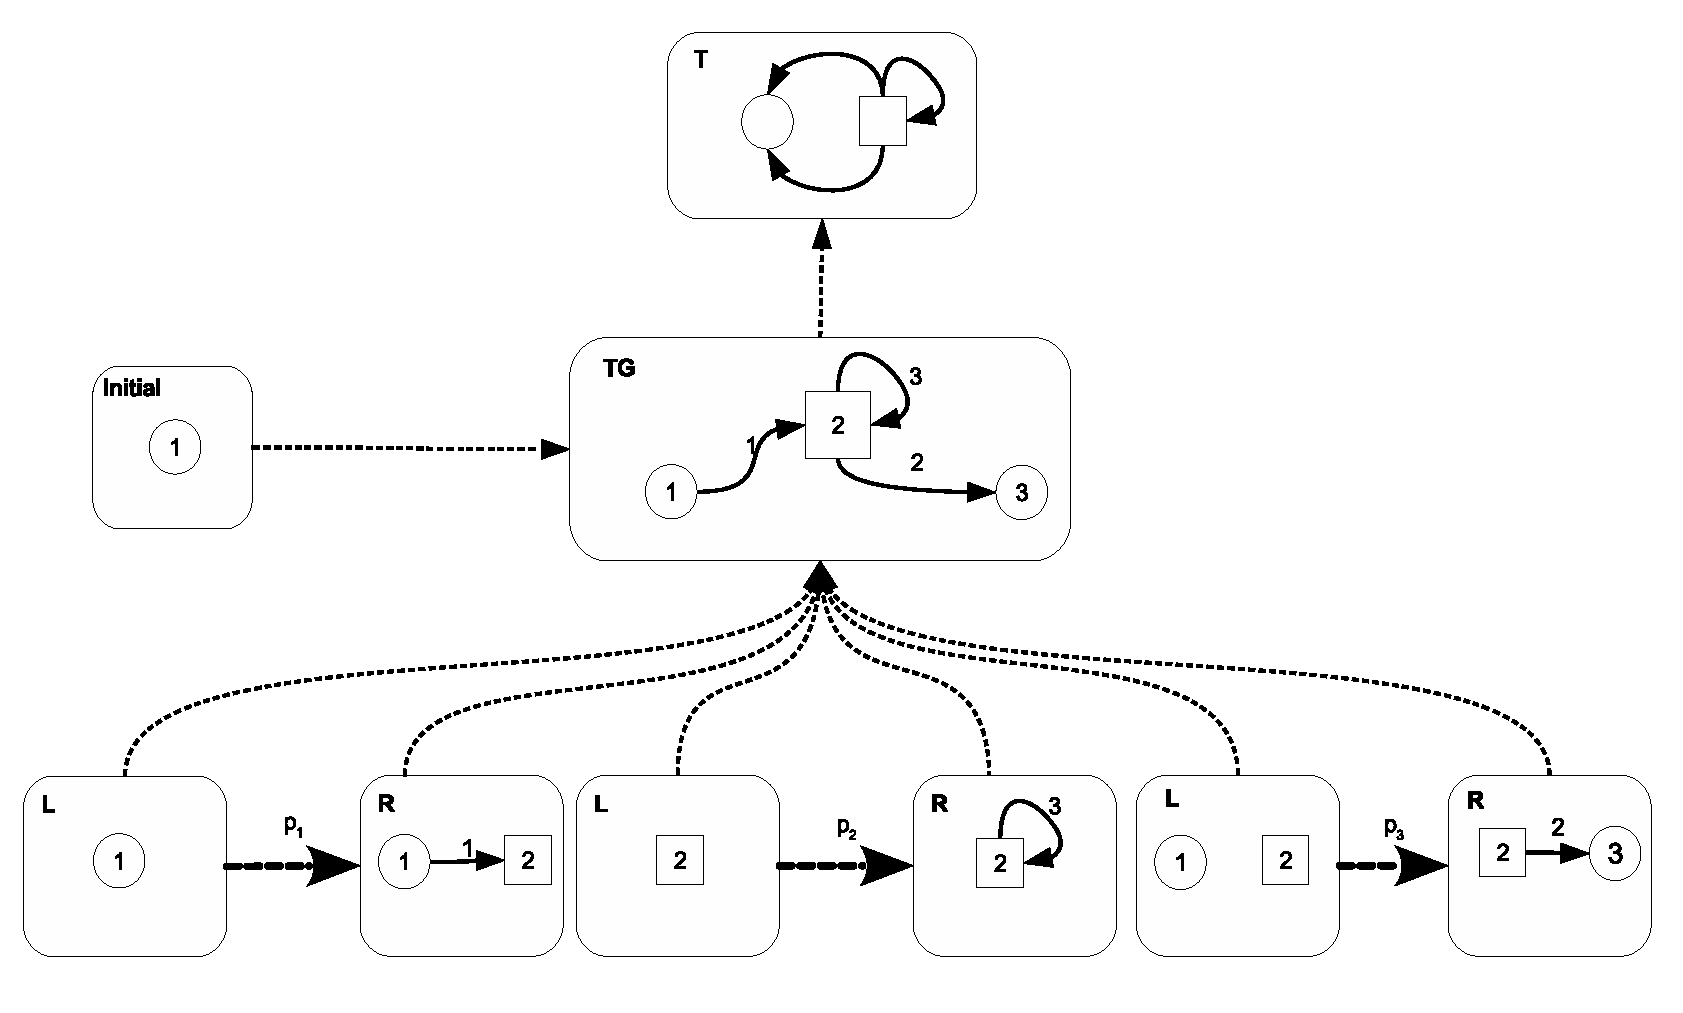
\includegraphics[scale=0.5]{images/process/core_graph/example}}}
    \caption{A grammar with a double-type graph that is also a core graph.}\label{fig:process:core-graph:example}
  \end{subfigure}

  \caption{Doubly-typed graph grammars}\label{fig:process:doubly-typed-grammars}
\end{figure}

\end{example}

\begin{notation}[Restriction to Image] Given an arbitrary morphism $f : A \rightarrow X$, we will denote as $f' : A \rightarrow X_{|A}$ the morphism derived from $f$ where $X_{|A}$ is the image of $f$.

  For two arbitrary morphisms $f : A \rightarrow X$ and $g : B \rightarrow X$, we will denote as $f' : A \rightarrow X_{|AB}$ and $g' : B \rightarrow X_{|AB}$ the morphisms derived from $f$ and $g$ where $X_{|AB}$ is the joint image of both $f$ and $g$.
\end{notation}

\begin{definition}[Strongly Safe (Doubly-Typed) Graph Grammars]\label{def:strongly-safe-grammar} Given \doublyTypedGraphGrammarCore{} a doubly-typed graph grammar, $GG$ is said to be \emph{strongly safe} if its double-type graph is also a core graph.

  Each rule in a strongly safe graph grammar is also called an \emph{action}. We say that an action $a$ creates an element $e$ iff $e \in R(a) - K(a)$. Similarly, $a$ deletes $e$ iff \mbox{$e \in L(a) - K(a)$}. Finally, if $e$ is present in $K(a)$, we say that $a$ preserves $e$.
\end{definition}

In the context of strongly safe graph grammars, we will use a slightly different interpretation of a graph transformation:
  
\begin{itemize} 
  \item Isolated actions are always applied over a subgraph of the core graph: the match of an action is equal to its pre-condition $pre_a : L \rightarrow C^T_{L_a}$, as well as the comatch is equal to its post-condition $post_a : R \rightarrow C^T_{R_a}$.

  \item When searching for conflicts (resp. dependencies) between two actions, the overlapping between them is the restricted image of their matches $E = C^T_{|L_1L_2}$ (resp. comatch and match $E = C^T_{|R_1L_2}$). The derived graphs are calculated accordingly when the DPO transformations exist, i.e. \mbox{$E \xRightarrow{a_1} H_1$} (resp. \mbox{$E \xRightarrow{a^{-1}_1} H_1$}), \mbox{$E \xRightarrow{a_2} H_2$}. Notice that, as the transformations are always concrete regarding the core
    graph, we have $H_1 \xhookrightarrow{} C^T, H_2 \xhookrightarrow{} C^T$.

  \item When searching for conflicts (resp. dependencies) between two actions $a_1,a_2$ with NACs, we check the NAC satisfiability only in the overlapping and the derived graphs rather than the entire core graph.
\end{itemize}

  By restricting the overlapping of actions to the images of their matches (resp. comatch and match) we consider only the local effects of these actions. Thus resulting in two properties of our interest: (1) We avoid dangling conditions with edges in the core graph that do not directly participate in the interaction of these actions. Similarly, (2) the NACs of these actions are not triggered by elements that, in despite of being present in the core graph, do not directly participate in the interaction of these two actions. These restrictions, together with the use of incremental NACs, allow us to locally compute the conflicts and dependencies for each pair of actions, without the necessity of dealing with global effects other actions might have.

\begin{remark}[Strongly Safe Grammars] Throughout the rest of this work, we will use only strongly safe grammars whose set $P$ of actions is finite and each action in $P$ is distinct from the others.

\hfill
\end{remark}

\begin{example}[Strongly Safe Graph Grammar] Figure~\ref{fig:process:core-graph:example} also depicts a strongly safe graph grammar as the double-type graph of the grammar is, in fact, a core graph.
\end{example}

\section{Relations within Strongly Safe Graph Grammars without NACs}

Given a strongly safe graph grammar, its core graph contains all elements used (created, read or deleted) during one possible execution of the grammar. Moreover, as each element has a unique origin, the core graph can be considered to contain the entire ``execution history'' of its underlying grammar.

We are here interested in some of the properties that can be found by looking at this history. Particularly, we want to define the kind of relations that exist among actions and elements, whether it is possible to find sequences in which all actions are applied and which graphs can be considered valid (reachable) by this grammar.

In~\cite{Ribeiro1996}, causal, conflict and occurrence relations for strongly safe graph grammars were defined. There, the graph transformation approach used was the \emph{Single Pushout} (SPO) without NACs. \cite{Corradini1996} also defined a different notion of causal relation, equivalent to the occurrence relation in the previous mentioned work, with respect to the DPO approach without NACs.

Both authors use these relations to find out whether all the actions of a strongly safe graph grammar are applicable and prove the above mentioned properties about them. However, these relations alone are not sufficient to prove such properties when the actions have NACs.

Here we recall the work of ~\cite{Corradini1996}, since it already uses the DPO approach, then extend it to create an equivalent notion of \emph{occurrence relation} that works for grammars in the DPO approach with NACs.

\begin{definition}[Causal Relation]\label{def:causal-relation} \emph{(This is the same causal relation defined in \cite{Corradini1996} for the DPO approach without NACs.)} Given  \doublyTypedGraphGrammarCore{} a strongly safe graph grammar, actions \mbox{$a_1, a_2 \in P, a_1 \ne a_2$} and an element \mbox{$e \in N(C^T) \cup E(C^T)$}, then:

  \begin{enumerate}
    \item If $a_1$ deletes $e$, then $e <_c a_1$.
    \item If $a_1$ creates $e$, then $a_1 <_c e$.
    \item If $a_1$ creates $e$ and $a_2$ preserves $e$, then $a_1 <_c a_2$.
    \item If $a_1$ preserves $e$ and $a_2$ deletes $e$, then $a_1 <_c a_2$. 
    \item The \emph{causal relation} $\leq_c$ of $P \cup N(C^T) \cup E(C^T)$ is the reflexive and transitive closure of $<_c$.
  \end{enumerate}\end{definition}

This relation represents conditions over creation, use (preservation) and deletion of elements by the actions used to characterize executions of the underlying rules. In any of the derivations represented by this strongly safe graph grammar, an action $a$ must occur after all actions that create the elements it preserves or deletes. Analogously, $a$ must occur before all actions that delete the elements created or preserved by it.

In \cite{Corradini1996} it is shown that if this relation is a \emph{partial order}, then any total order with respect to it is a sequencing in which all productions of the underlying grammar are applicable.

\begin{example}[Causal Relation in Grammars without NACs]\label{ex:process:existential-relation} Given the strongly safe grammar corresponding to the core and initial graphs in Figure~\ref{fig:process:existential-relation:core-graph} and the set of rules in Figure~\ref{fig:process:existential-relation:example}, we have that:

\begin{itemize}
  \item $a_1 <_c \triangle_2$
  \item $a_2 <_c \Square_1$ and $a_2 <_c$ $\curvearrowleft_1$
  \item $a_3 <_c$ $\curvearrowleft_2$
  \item $a_2 <_c a_1$ by creation/preservation of $\Square_1$
\end{itemize}

  The causal relation for this grammar is (without the pairs due to reflexivity): $a_1 \leq_c \triangle_2$, $a_2 \leq_c \Square_1$, $a_2 \leq_c$ $\curvearrowleft_1$, $a_3 \leq_c$ $\curvearrowleft_2$, $a_2 \leq_c a_1$, $a_2 \leq_c \triangle_2$. Notice that the only pair in this relation where both elements are actions is \mbox{$a_2 \leq_c a_1$}, therefore, we have that all actions in this grammar can be applied as long as $a_2$ is applied before $a_1$ ($a_2$ crates the element $\Square_1$
  which is necessary for $a_1$ to be applied). In particular, the following sequences of actions are valid and lead to the same resulting graph: $[a_2,a_1,a_3],[a_2,a_3,a_1],[a_3,a_2,a_1]$.

\begin{figure}[!ht]
  \centering
  \begin{subfigure}[t]{.5\textwidth}
    \centerline{\fbox{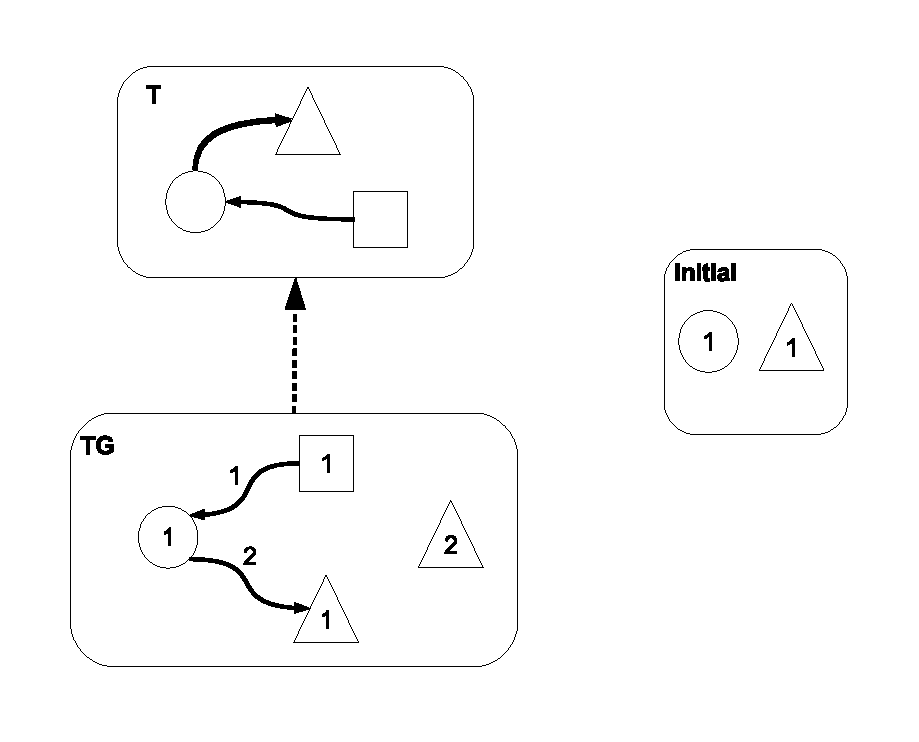
\includegraphics[scale=0.6]{images/process/existential-relation/core-graph}}}
    \caption{Core and initial graphs}\label{fig:process:existential-relation:core-graph}
  \end{subfigure}
  \begin{subfigure}[t]{.5\textwidth}
    \centerline{\fbox{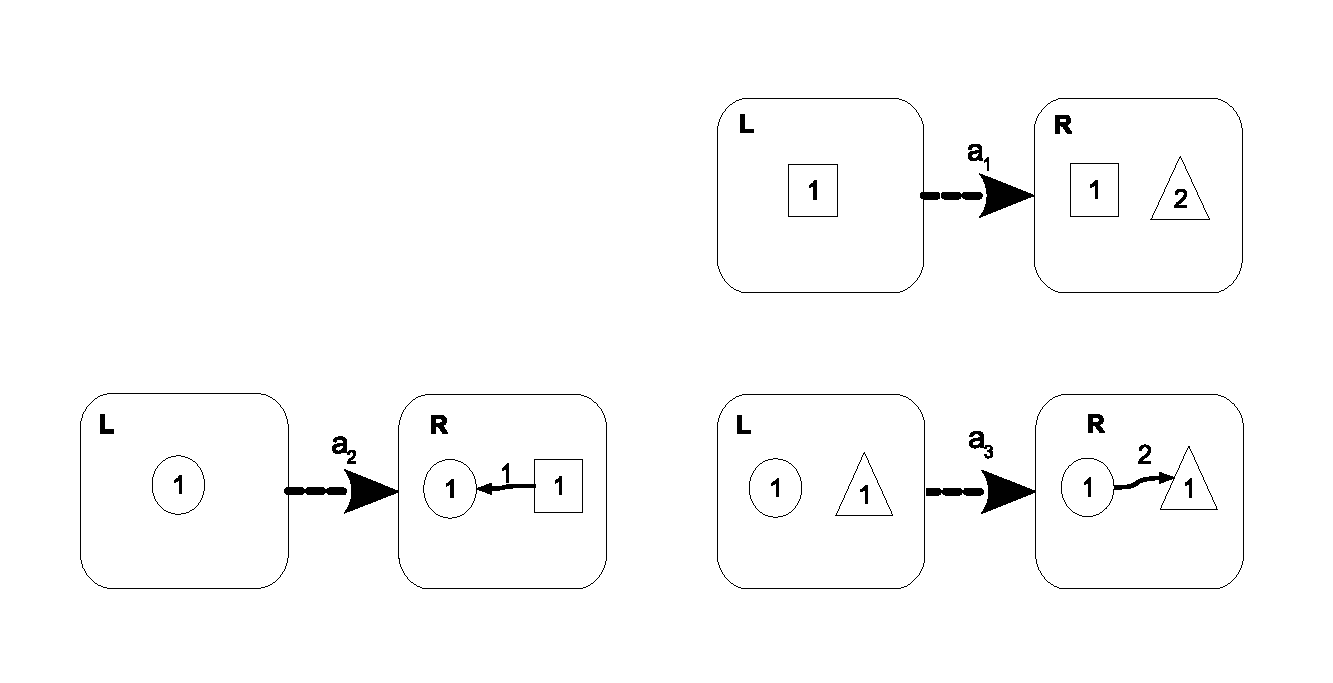
\includegraphics[scale=0.6]{images/process/existential-relation/example}}}
    \caption{A strongly safe grammar without NACs}\label{fig:process:existential-relation:example}
  \end{subfigure}
  \begin{subfigure}[t]{.5\textwidth}
    \centerline{\fbox{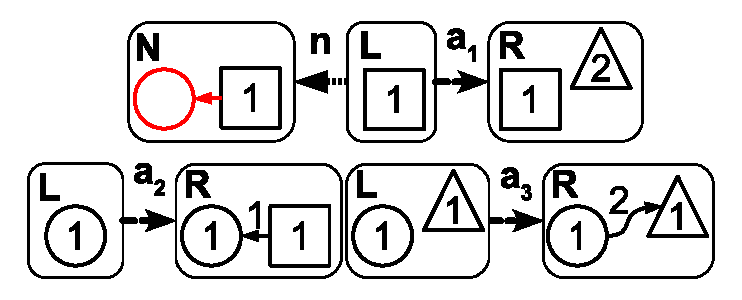
\includegraphics[scale=0.6]{images/process/existential-relation/example-nacs}}}
    \caption{A strongly safe grammar with NACs}\label{fig:process:existential-relation:example-nacs}
  \end{subfigure}
  \stepcounter{doubly-typed-grammar-counter}
  \caption{Strongly safe grammar GG\arabic{doubly-typed-grammar-counter}}\label{fig:process:existential-relation}
\end{figure}
\end{example}

The same definition can be attempted in a strongly safe grammar where actions are equipped with NACs. However, as shown in examples~\ref{ex:process:existential-relation-fail} and \ref{ex:process:existential-relation-fail2}, it lacks the same properties as in the case without NACs.

\begin{example}[Causal Relation in Grammars with NACs]\label{ex:process:existential-relation-fail}Consider the strongly safe grammar corresponding to the core and initial graphs in Figure~\ref{fig:process:existential-relation:core-graph} and the set of rules in Figure~\ref{fig:process:existential-relation:example-nacs}.

We have the same causal relation as the one presented in Example~\ref{ex:process:existential-relation}, since the structure of the actions is the same in both examples, except for the NAC in the action $a_1$ on Figure~\ref{fig:process:existential-relation:example-nacs}. In this example, we still have that $a_2$ must be applied first in order for $a_1$ to be applied. However, besides creating the $\Square_1$ needed for $a_1$, $a_2$ also creates a $\curvearrowleft_1$ from $\Square_1$ to
  $\Circle_1$ which is a pattern forbidden by the NAC of $a_1$. Therefore, we have that $a_2$ also causes a \emph{produce-forbid} conflict with $a_1$. Moreover, $a_3$ is the only other action in this grammar and it does not delete any element that could undo the forbidden pattern. Thus, there is no possible way of applying all actions of this grammar, even though the causal relation is a partial order.\end{example}

\iffalse
The next \emph{unconditional relations} are equivalent to the \emph{causal dependency} and \emph{weak conflict} relations presented at~\cite{Ribeiro1996}, but for the DPO rather than the SPO approach. These relations will be used as basis to the \emph{conditional relations} that will be later defined for conflicts and dependencies with NACs.

Regarding both unconditional and conditional dependency relations, their definitions are based on the following intuition:

\begin{intuition} An action $a_1$ is a direct cause of an action $a_2$ if either $a_1$ creates some element that is needed by $a_2$ (unconditional causal dependency) or $a_1$ deletes an element that is both forbidden by a NAC of $a_2$ and existent before the application of $a_2$ (conditional causal dependency). In both cases, we have that $a_2$ can only happen after $a_1$ has been applied.
\end{intuition}

\begin{figure}[!ht]
  \centering
  \begin{subfigure}[t]{.5\textwidth}
    \centerline{\fbox{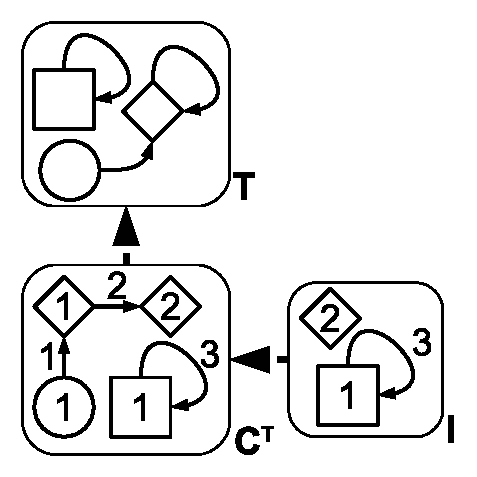
\includegraphics[scale=0.5]{images/process/unconditional-relation/core-graph}}}
    \caption{Core and initial graphs}\label{fig:process:unconditional-relation:core-graph}
  \end{subfigure}

  \begin{subfigure}[t]{.5\textwidth}
    \centerline{\fbox{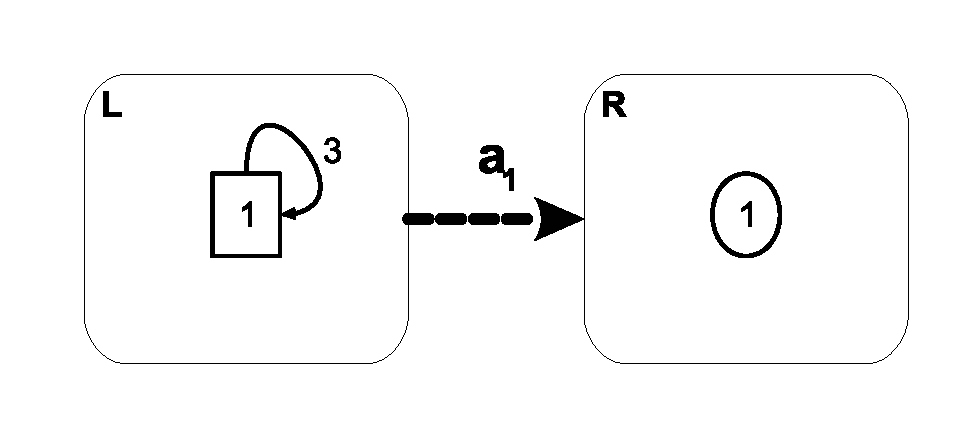
\includegraphics[scale=0.45]{images/process/unconditional-relation/a1}}}
    \caption{Action $a_1$}\label{fig:process:unconditional-relation:a1}
  \end{subfigure}%
  \begin{subfigure}[t]{.5\textwidth}
    \centerline{\fbox{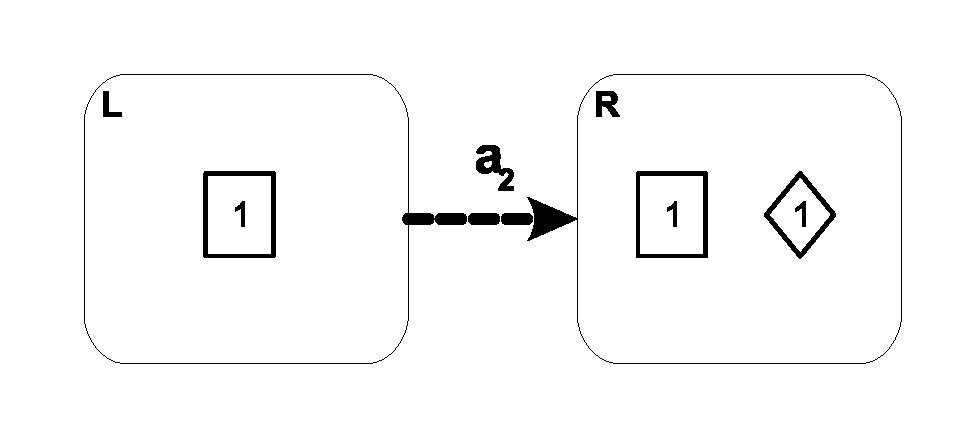
\includegraphics[scale=0.45]{images/process/unconditional-relation/a2}}}
    \caption{Action $a_2$}\label{fig:process:unconditional-relation:a2}
  \end{subfigure}

  \begin{subfigure}[t]{.5\textwidth}
    \centerline{\fbox{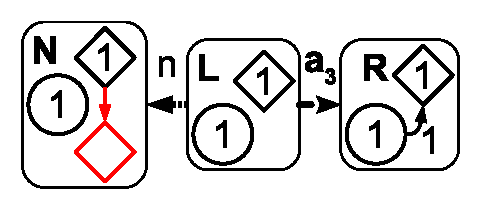
\includegraphics[scale=0.45]{images/process/unconditional-relation/a3}}}
    \caption{Action $a_3$}\label{fig:process:unconditional-relation:a3}
  \end{subfigure}%
  \begin{subfigure}[t]{.5\textwidth}
    \centerline{\fbox{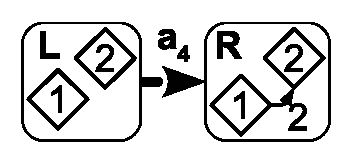
\includegraphics[scale=0.45]{images/process/unconditional-relation/a4}}}
    \caption{Action $a_4$}\label{fig:process:unconditional-relation:a4}
  \end{subfigure}
  \stepcounter{doubly-typed-grammar-counter}
  \caption{Strongly safe grammar GG\arabic{doubly-typed-grammar-counter}}\label{fig:process:unconditional-relation}
\end{figure}

\begin{definition}[Unconditional Causal Dependency Relation\footnote{Also called Produce-Use Relation.}]\label{def:unconditional-causal-dependency} Given \doublyTypedGraphGrammarCore{} a strongly safe graph grammar. Let $a_1, a_2 \in P$, $a_1 \ne a_2$, \mbox{$e_1, e_2 \in $ \coreGraph{}} and $e_1 \ne e_2$. Then: 

  \begin{enumerate}
    \item The action $a_2$ is \emph{directly causally dependent} on $a_1$, written $a_1 <_{pu} a_2$, iff \mbox{$\not\exists h_{21} : L_2 \rightarrow D_1$ s.t. \mbox{$d_1 \circ h_{21} = pre_2$}}, where the two squares are pushouts and $C^T_{|R_1L_2}$ ($C^T$ restricted to the joint image of $post_1$ and $pre_2$) satisfies the NACs for $a_2$ and $a_1^{-1}$.

\diagram{
   & & N_1^{-1} & & N_2 & & \\
      L_1 & K_1\ar[d]\ar[l]\ar[r] & R_1\ar[u]\ar[dr]_{post_1} & & L_2\ar[u]\ar@{.>}@/_1.1pc/[dlll]|{|}_<<<<{h_{21}}\ar[dl]^{pre_2} & K_2\ar[l]\ar[r]\ar[d] & R_2\\
       & D_1\ar@{^{(}->}[rr]_{d_1} & & C^T_{|R_1L_2} & & D_2\ar@{_{(}->}[ll]^{e_2} &}

   \item The \emph{causal dependency relation between actions} $\leq_{pu}$ of $P$ is the reflexive and transitive closure of the direct causal dependency.
   \item The element $e_2$ is \emph{directly causally dependent} on $e_1$, written $e_1 <_{pu} e_2$, iff there is an action $a_1 \in P$ such that $a_1$ deletes $e_1$ and creates $e_2$.
   \item The \emph{causal dependency relation between elements} $\leq_{pu}$ of $N(C^T) \cup E(C^T)$ is the reflexive and transitive closure of the direct causal dependency.
   \item The \emph{unconditional causal dependency relation} of a strongly safe grammar is defined as the transitive and reflexive closure of the union of both relations $\leq_{pu}$ for $P$ and $N(C^T) \cup E(C^T)$.
  \end{enumerate}
\end{definition}

\begin{example}[Unconditional Dependency Example]Figure~\ref{fig:process:unconditional-relation:dependency} \tinytodo{review the names of the graphs} shows a produce-use between the actions $a_2$ and $a_4$ of the strongly safe grammar depicted in Figure~\ref{fig:process:unconditional-relation}.

  This conflict occurs due to the fact that, besides both actions have valid graph transformations (they satisfy the rewriting conditions for the overlapping on $C^T$ restricted do the image of $post_2$ and $pre_4$ and none of them has any NACs), it is not possible to find a morphism from $L_4$ to $D_2$ satisfying the conditions on Definition~\ref{def:unconditional-causal-dependency}.

\begin{figure}[!ht]
  \centering
  \fbox{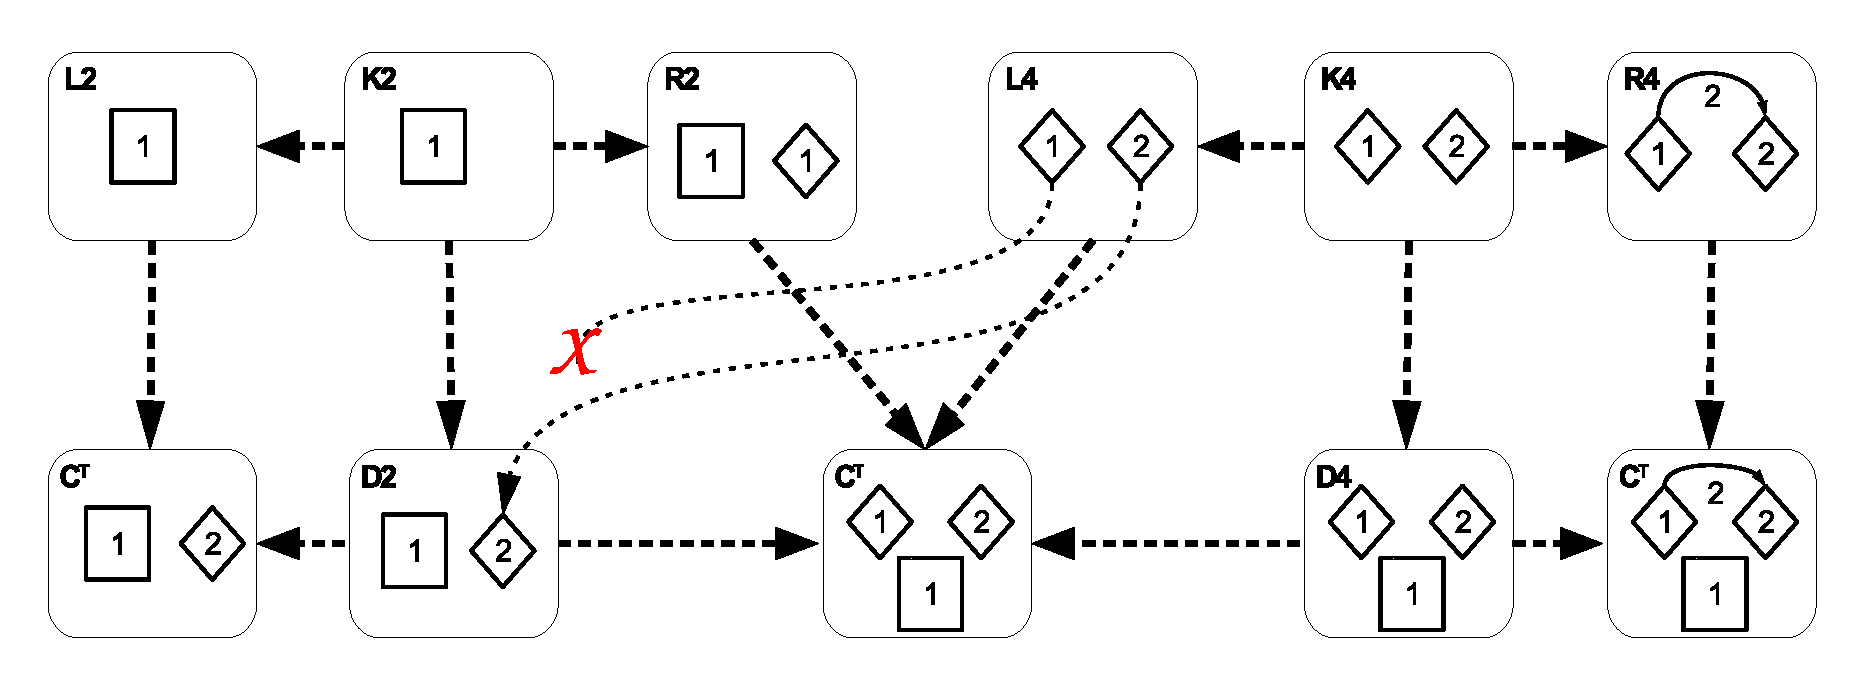
\includegraphics[scale=0.48]{images/process/unconditional-relation/dependency}}
  \caption{Unconditional causal dependency situation}\label{fig:process:unconditional-relation:dependency}
\end{figure}
\end{example}

Regarding both unconditional and conditional weak conflict relations, their definitions are based on the following intuition:

  \begin{intuition} An action $a_1$ is in \emph{weak} conflict with an action $a_2$ if either $a_1$ deletes something that is needed by $a_2$ to be applied (unconditional weak conflict) or creates something that is both forbidden by a NAC of $a_2$ and not deleted before the application of $a_2$ (conditional weak conflict). In both cases, we have that $a_2$ can not be applied once $a_1$ has been applied, in other words, $a_2$ can only be applied before $a_1$.
\end{intuition}

\begin{definition}[Unconditional Weak Conflict Relation\footnote{Also called Delete-Use Relation.}]\label{def:unconditional-conflict} Given \doublyTypedGraphGrammarCore{} a strongly safe graph grammar. Let $a_1, a_2 \in P$, $a_1 \ne a_2$, \mbox{$e_1, e_2 \in $ \coreGraph{}} and $e_1 \ne e_2$. Then: 

  \begin{enumerate}
    \item The action $a_1$ is in \emph{direct weak conflict} with $a_2$, written $a_2 <_{du} a_1$, iff \mbox{$\not\exists h_{21} : L_2 \rightarrow D_1$} s.t. \mbox{$d_1 \circ h_{21} = pre_2$}.

      \diagram{
          & & N_1 & & N_2 & & \\
        R_1 & K_1\ar[l]\ar[r]\ar[d] & L_1\ar[u]\ar[dr]_{pre_1} & & L_2\ar[u]\ar[dl]^{pre_2}\ar@{.>}@/_1.1pc/[dlll]|{|}_<<<<{h^{21}} & K_2\ar[l]\ar[r]\ar[d] & R_2\\
       & D_1\ar[rr]_{d_1} & & C^T_{|L_1L_2} & & D_2\ar[ll] &}
   \item The \emph{weak conflict relation between actions} $\leq_{du}$ of $P$ is the reflexive and transitive closure of the direct weak conflict.
   \item The element $e_2$ is \emph{in direct weak conflict} with $e_1$, written $e_2 <_{du} e_1$, iff there are actions $a_1$ and $a_2$ that respectively create $e_1$ and $e_2$ and $a_2 \leq_{du} a_1$.
   \item The \emph{weak conflict relation between elements} $\leq_{du}$ of $N(C^T) \cup E(C^T)$ is the reflexive and transitive closure of the direct weak conflict.
   \item The \emph{weak conflict relation} of a strongly safe grammar is defined by transitive and reflexive closure of the unions of relations $\leq_{du}$ for $P$ and $N(C^T) \cup E(C^T)$.

  \end{enumerate}
\end{definition}

\begin{example}[Unconditional Weak Conflict Example] Figure~\ref{fig:process:unconditional-relation:conflict} shows a delete-use between the actions $a_1$ and $a_2$ of the strongly safe grammar depicted in Figure~\ref{fig:process:unconditional-relation}.

  Again, both actions have valid graph transformations, now for the overlapping of $pre_1$ and $pre_2$ on $C^T$, but it is not possible to find a morphism from $L_2$ to $D_1$ satisfying the conditions on Definition~\ref{def:unconditional-conflict}.
\begin{figure}[!ht]
  \centering
  \fbox{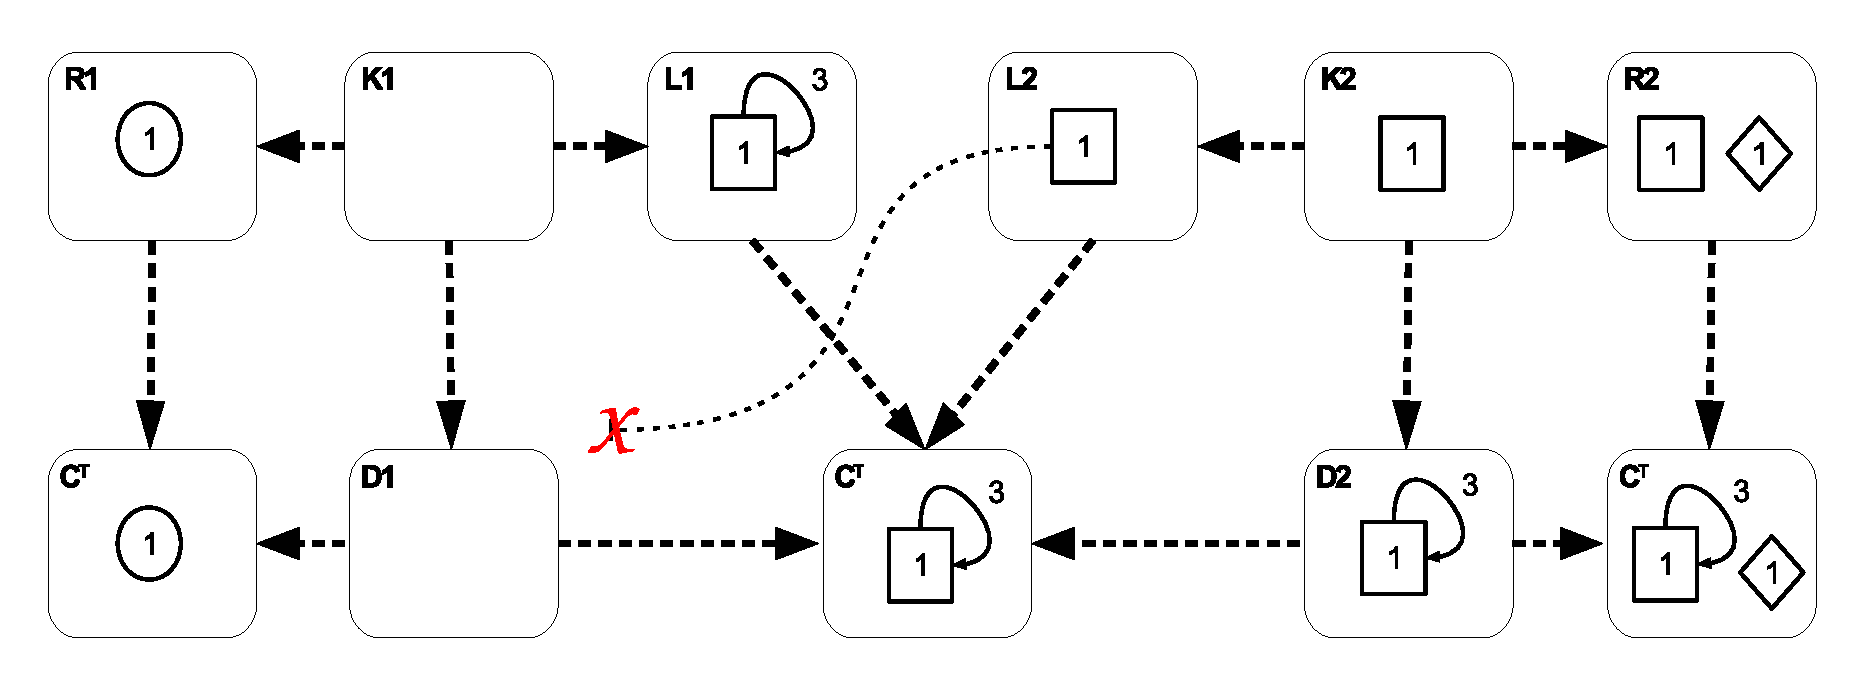
\includegraphics[scale=0.48]{images/process/unconditional-relation/conflict}}
  \caption{Unconditional weak conflict situation}\label{fig:process:unconditional-relation:conflict}
\end{figure}
\end{example}

\begin{definition}[Unconditional Occurrence Relation] Given \doublyTypedGraphGrammarCore{} a strongly safe graph grammar, let $\leq_{pu}$ and $\leq_{du}$ be the unconditional dependency and unconditional weak conflict relations of this grammar for $P \cup N(C^T) \cup E(C^T)$. Then the \emph{unconditional occurrence relation} of GG is the reflexive and transitive closure of \mbox{$\leq_{pu} \cup \leq_{du}$}.
\end{definition}

Similarly to the existential relation,~\cite{Ribeiro1996} proved that if this relation is a partial order, then it is possible to apply all actions of its underlying grammar in any total order that respects the partial order. Again, this condition is not sufficient if the rules may be equipped with NACs, as it was also shown to be equivalent to the existential relation.

\fi

\begin{example}[Causal Relation in Grammars with NACs]\label{ex:process:existential-relation-fail2} Consider the strongly safe grammar depicted on Figure~\ref{fig:process:unconditional-relation}, for which we have $a_1 \leq_c a_3$, $a_2 \leq_c a_3$, $a_2 \leq_c a_4, a_2 \leq_c a_1$ as causal relation: in order to know if all the actions of a strongly safe grammar without NACs can be applied, it would be sufficient to check whether the causal relation is a partial order.

\begin{figure}[!ht]
  \centering
  \begin{subfigure}[t]{.5\textwidth}
    \centerline{\fbox{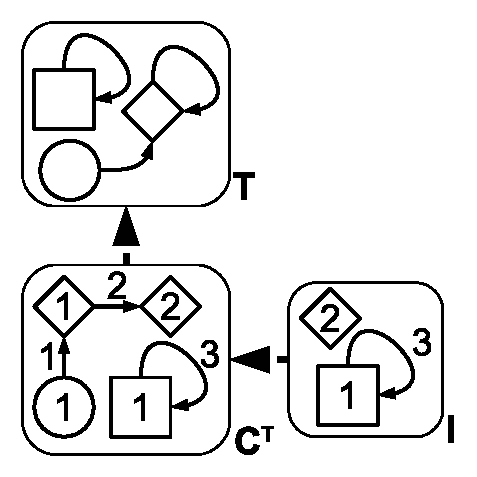
\includegraphics[scale=0.5]{images/process/unconditional-relation/core-graph}}}
    \caption{Core and initial graphs}\label{fig:process:unconditional-relation:core-graph}
  \end{subfigure}

  \begin{subfigure}[t]{.2\textwidth}
    \centerline{\fbox{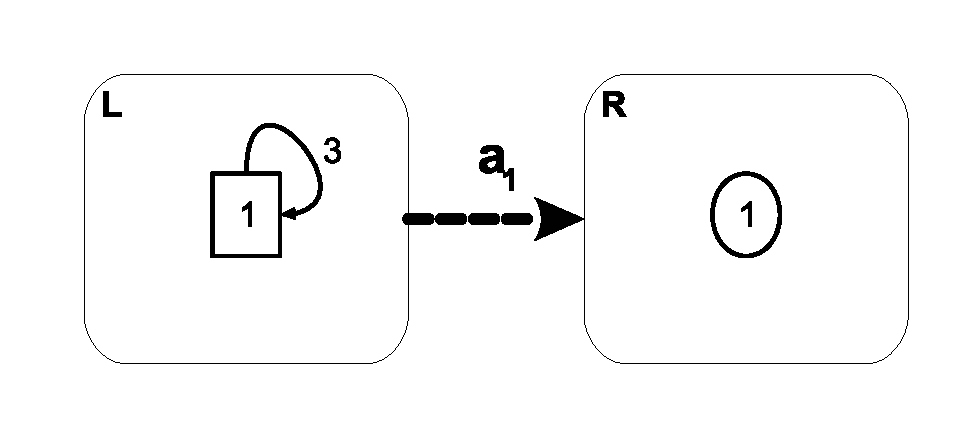
\includegraphics[scale=0.5]{images/process/unconditional-relation/a1}}}
    \caption{Action $a_1$}\label{fig:process:unconditional-relation:a1}
  \end{subfigure}%
  \begin{subfigure}[t]{.2\textwidth}
    \centerline{\fbox{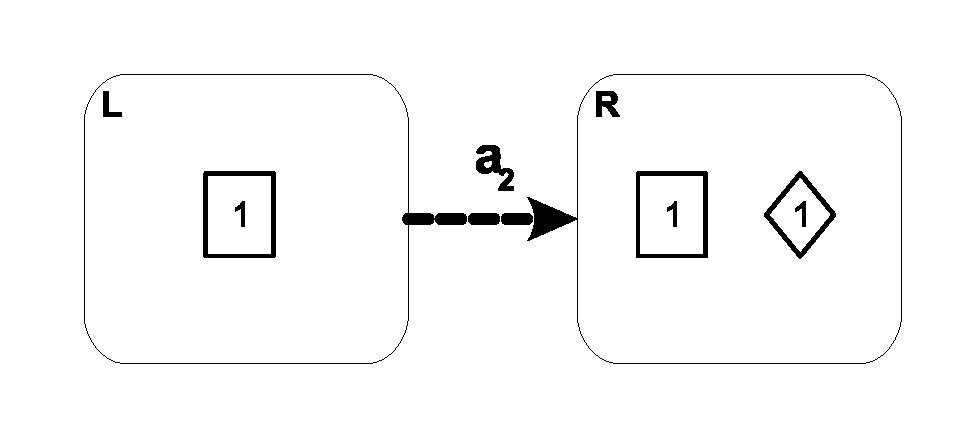
\includegraphics[scale=0.5]{images/process/unconditional-relation/a2}}}
    \caption{Action $a_2$}\label{fig:process:unconditional-relation:a2}
  \end{subfigure}%
  \begin{subfigure}[t]{.3\textwidth}
    \centerline{\fbox{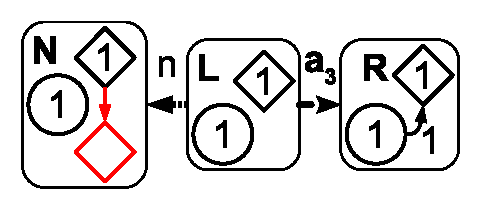
\includegraphics[scale=0.5]{images/process/unconditional-relation/a3}}}
    \caption{Action $a_3$}\label{fig:process:unconditional-relation:a3}
  \end{subfigure}%
  \begin{subfigure}[t]{.2\textwidth}
    \centerline{\fbox{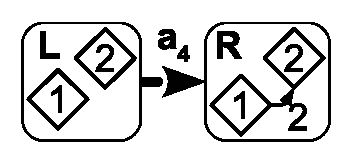
\includegraphics[scale=0.5]{images/process/unconditional-relation/a4}}}
    \caption{Action $a_4$}\label{fig:process:unconditional-relation:a4}
  \end{subfigure}
  \stepcounter{doubly-typed-grammar-counter}
  \caption{Strongly safe grammar GG\arabic{doubly-typed-grammar-counter}}\label{fig:process:unconditional-relation}
\end{figure}

  In particular, if we do not consider NACs for the grammar in Figure~\ref{fig:process:unconditional-relation}, any total order of actions compatible with the partial order of the causal relation would be a valid sequencing of this grammar. As an example, $[a_2, a_1, a_3, a_4]$ and $[a_2, a_4, a_1, a_3]$ are valid sequences (without NACs) for this grammar. 

  However, not all previous sequences are valid when NACs come into play. Specifically, $[a_2, a_4, a_1, a_3]$ is not valid, because if $a_4$ is applied before $a_3$ it creates $\curvearrowleft_2$, triggering the NAC of $a_3$ which can no longer be applied. 
\end{example}
\hide{
\begin{remark}[Causal and Unconditional Occurrence Relations] Since the \emph{causal} and \emph{unconditional occurrence relations} where shown to be equivalent by~\cite{Ribeiro1996}, we will only one of them, the \emph{causal relation}, as the standard relation without without NACs from now on, as it was originally defined for DPO grammars.

  However, we were heavily inspired by the structure of the \emph{unconditional causal dependency} and \emph{unconditional weak conflict relations} to define the relations with NACs.
\end{remark}}

\section{Relations within Strongly Safe Graph Grammars with NACs}

It is important to notice that the causal relation presented in the previous section is always concrete. This means that if an action is dependent on (resp. conflicting with) another one, it happens because one of them creates (resp. deletes) at least one of the concrete elements necessary for the other to be applied (resp. prevented of being applied).

Moreover, the causal relation must always be respected whenever we try to find a total order in which all the actions of a strongly safe grammar are applicable. Nonetheless, for grammars equipped with NACs it is necessary to include the conflicts and dependencies created by NACs in this relation.

This inclusion of conflicts and dependencies induced by NACs gives rise to a new problem: we can not just add those conflicts and dependencies directly into the causal relation because they are \textit{potential} instead of concrete. They may or may not happen depending on which specific total ordering of application (among all possibilities) was performed. Therefore, we need a way to identify under which conditions these potential conflicts (resp. dependencies) will appear, in order to know which among the possible total orderings also respect the restrictions imposed by NACs.

\begin{example}[Interaction between causal relation and NACs]
Let $a_1, a_2, a_3$ be three actions of the same strongly safe grammar. 
  Suppose that $a_1$ creates elements used by $a_2$ and $a_2$ creates elements used by $a_3$, therefore by the causal relation we know that $a_1 \leq_c a_2 \leq_c a_3$. 
  Now suppose that when $a_2$ is applied, it creates an element that would be forbidden by a NAC of $a_1$ and also that $a_3$ deletes this element. 
  Following the classical notions of dependency and conflict of graph grammars with NACs, as shown in  definitions~\ref{def:classic-dependency} and~\ref{def:classic-conflict}, $a_2$ would cause a (potential) produce-forbid conflict on $a_1$, thus $a_1$ should be applied before $a_2$ $(a_1 <_{pf} a_2)$. Likewise, $a_1$ would be (potentially) dependent by delete-forbid on $a_3$, consequently $a_3$ should be applied before $a_1$ $(a_3 <_{df} a_1)$. By adding these produce-forbid and delete-forbid directly into the causal relation we would have the situation depicted in Figure~\ref{fig:process:order:occurrence-relation-fail}. It is easy to see that the resulting relation is not a partial order, therefore there can be no total ordering for this set of actions.
\begin{figure}[!ht]
  \centering
  \fbox{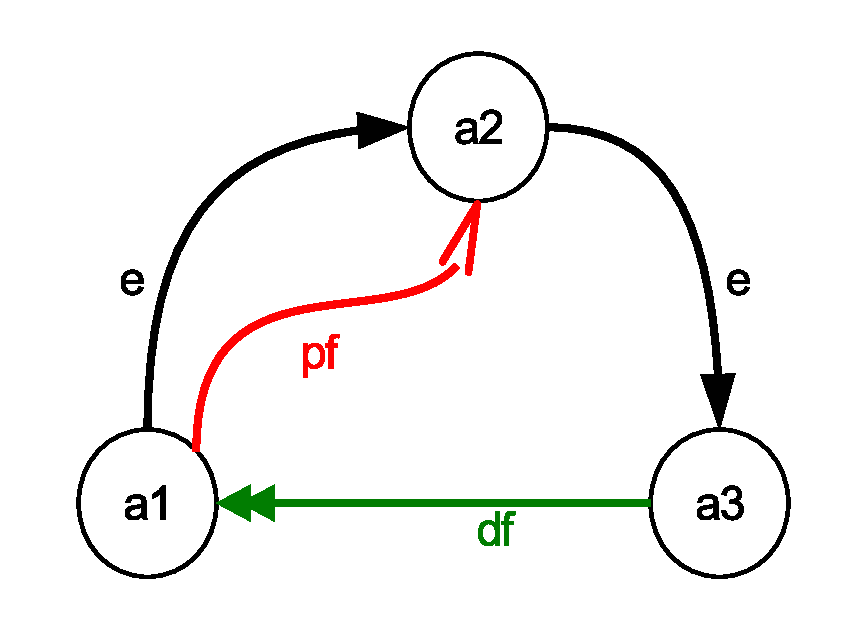
\includegraphics[scale=1]{images/process/order/occurrence-relation-fail}}
  \caption{Graph of relations}\label{fig:process:order:occurrence-relation-fail}
\end{figure}

Notwithstanding, by analysing the causal relation we can affirm that this configuration ensures that neither the conflict nor the dependency will ever exist in any concrete execution of this grammar. For the conflict, this happens because $a_2$ can only happen after $a_1$, thus the element forbidden by the NAC of $a_1$ can only exist after $a_1$ itself was already applied. Likewise, the dependency that is identified because $a_3$ deletes the element that would be forbidden by the NAC of $a_1$
  does not exist either, because $a_1$ was executed before its triggering element even existed.
\end{example}

\begin{definition}[Conflict and Dependency Characterization]\label{def:conflict-dependency-characterization} Given a strongly safe graph grammar \doublyTypedGraphGrammarCore{}, every conflict (resp. dependency) induced by NACs between two distinct actions $a_i, a_j \in P$ is said to be \emph{potential} (as we initially do not know whether this particular situation will occur during an execution of the underlying grammar). %Each potential conflict (resp. dependency) can be characterized according to how it relates to the overall grammar execution.

    Given a potential conflict (resp. dependency) situation in a strongly safe grammar, we say that it is:
    \begin{itemize}
      \item \emph{concrete}, if it always occur in any execution of the grammar;
      \item \emph{abstract}, if it occurs only in some of the executions;
      \item \emph{non-existent}, if it is never possible for it to occur in any execution of the grammar.
    \end{itemize}
\end{definition}

\begin{definition}[Abstract Conflicts and Dependencies] Given a strongly safe graph grammar \doublyTypedGraphGrammarCore{}, an abstract conflict/dependency is a tuple of distinct actions $t = (a_i,a_j,a_k)$. In any total ordering $<_t$ of actions in $P$, $t$ restricts the application of $a_i$ such that either $a_i <_t a_j$ or $a_k <_t a_i$.

\hfill
\end{definition}

The definition of abstract conflicts and dependencies translates to ``the action $a_i$ can only be applied either before $a_j$ or after $a_k$, but never in between their applications''. This situation models the following configuration of actions: $a_j$ creates an element $x$ which triggers a NAC of $a_i$, while $a_k$ deletes this same element. Therefore, $a_i$ can not be applied while $x$ exists.

We already know that at least the causal relation must be a partial order in order to be possible to apply all the actions of a grammar. Nevertheless, the following problem remains to be solved:

\begin{intuition}
  \emph{Given a strongly safe grammar \doublyTypedGraphGrammarCore{} with at least two actions $a_1, a_2 \in P$ in a potential delete-forbid or produce-forbid situation, under which circumstances this dependency or conflict exists and must be considered in the actions application ordering?}
\end{intuition}

In the following, we categorize these conflicts and dependencies using their triggering elements and pertinence of these elements into the causal relation in order to address this problem.

\begin{definition}[Delete-Forbid Relation in Strongly Safe Graph Grammars]\label{def:delete-forbid-strong} Let \doublyTypedGraphGrammarCore{} be a strongly-safe graph grammar, where $P$ is a set of actions with incremental, non-trivially triggered NACs only.

\diagram{
  \mathbf{a_1} & & N^{-1}_1 & & N_2\ar@{.>}@/_1.1pc/[ddllll]_<<<<{q} & & \mathbf{a_2}\\
  L_1\ar[d] & K_1\ar[d]\ar[l]\ar[r] & R_1\ar[u]^{n_1}\ar[dr]_{post_1} & & L_2\ar[u]_{n_2}\ar@{.>}@/_1.1pc/[dlll]_<<<<{h_{21}}\ar[dl]^{pre_2} & K_2\ar[l]\ar[r]\ar[d] & R_2\\
     H_1 & D_1\ar[rr]_{d_1}\ar[l]^{e_1} & & C^T_{|R_1L_2} & & D_2\ar[ll] &}
\hfill

  Let $a_1, a_2 \in P$ be in a potential delete-forbid dependency according to the diagram above, where $a_1$ deletes from graph $H_1$ an element $x \in N($\coreGraph$) \cup E($\coreGraph$)$ which is the triggering element of a NAC $N_2$ of $a_2$ for the extended match $e_1 \circ h_{21}$. This delete-forbid dependency is:

\begin{itemize}
  \item \emph{concrete}: iff $(x \leq_c a_2) \lor (x \in I^{C^T})$.%, therefore we have $a_1 <_{df} a_2$
  \item \emph{abstract}: iff $(\exists a_3 \in P \mid x \in R_3 - K_3)$ $\land$ $(x \not\leq_c a_2)$ $\land$ $(a_2 \not\leq_c x)$.%, thus $a_2 \not\in [a_3 \ldots a_1]$;
  \item \emph{non existent}: otherwise.
\end{itemize}

  If the above dependency is characterized as concrete, we have that \mbox{$a_1 <_{df} a_2$}. If it is abstract, $t_{df} = (a_2, a_3, a_1)$ is is the set of abstract conflicts and dependencies of the grammar $GG$. If it is non existent, the dependency is simply discarded in further analysis, since the orderings of execution are not affected by it.

\hide{Two elements $x, y \in N(C^T) \cup E(C^T)$ are in a delete-forbid dependency if there are actions $a_1,a_2$ such that (1) $a_1 <_{df} a_2$ and (2) $a_1$ creates $x$ and $a_2$ creates $y$. In this case use say that $x <_{df} y$.

  The delete-forbid between two elements has the same quality (concrete, abstract, non existent) as the one between the actions involved in this dependency.}
\end{definition}

According to our classification, we have that if a delete-forbid dependency is concrete, i.e. $a_i <_{df} a_j$, then we can only consider total orderings of $\leq_c$ where $a_i < a_j$. For the abstract case, we can only consider total orderings of $\leq_c$ where $a_i < a_j$ or $a_k < a_j$. If it is non existent there is no need to impose any new restrictions over the ordering of $\leq_c$. Thus, we need to demonstrate that:

\begin{thm} For each potential \emph{delete-forbid} in a strongly safe graph grammar, definition~\ref{def:delete-forbid-strong} correctly classifies these dependencies.
\end{thm}

\begin{proof} Given actions $a_1,a_2 \in P$ in a potential \emph{delete-forbid} where $a_1$ deletes an element $x \in C^T$ which is also the triggering element of a NAC in $a_2$. The following situations are possible:
\hfill
\begin{description}[style=nextline,leftmargin=*]

  \item [Triggering element is present on the initial graph:]
Let $x$ be an element which is not created by any action in $P$, meaning that $x$ is present on the initial graph: $x \in I^{C^T}$. In such configuration, the delete-forbid is \emph{concrete}, given that $x$ exists before the application of $a_2$ (or any other action), preventing the application of the action until it gets deleted. Therefore, we have $a_1 <_{df} a_2$.

  \item [Triggering element is related to the action:] If $a_2 \leq_c x$, it means that $x$ was either created by $a_2$ or by another action that must to occur after $a_2$. In this configuration the delete-forbid dependency is \emph{non existent} as the element $x$ can not exist to trigger $N_2$ before $a_2$ was already applied.

    On the other hand, if $x \leq_c a_2$, it means that $x$ must exist at some moment before $a_2$ is applied. In this configuration, we have that $x$ must be deleted in order for $a_2$ to be applied. Since $a_1$ is the only action that deletes $x$ (otherwise the underlying grammar would not be a strongly safe grammar) this delete-forbid is \emph{concrete} and we have that $a_1 <_{df} a_2$.

\item [Triggering element is not related to the action:]
  Let $x$ be not related to $a_2$, but created by a third action $a_3 \in P$ (notice that in this configuration we have that $a_3 <_{c} a_1$).

    If $a_3$ is not related to $a_2$, in which case we have that $a_1$ and $a_2$ \emph{would be} in a concrete delete-forbid dependency if $a_3$ were applied before $a_2$. On the other hand, the same dependency \emph{would be} non existent if $a_3$ were applied after $a_2$. This situation depicts an \emph{abstract} produce-forbid dependency as we have that either $a_1 <_{df} a_2$ or $a_2 < a_3$ are possible. Therefore $(a_2,a_3,a_1)$ is an abstract dependency.

  Finally, if $a_3$ is related to $a_2$, then $a_2$ is related to $x$, as $a_3$ creates $x$, which corresponds to our second case.
\end{description}
\end{proof}

\begin{definition}[Produce-Forbid Relation in Strongly Safe Graph Grammars]\label{def:produce-forbid-strong} Given \doublyTypedGraphGrammarCore{} a strongly safe graph grammar, where $P$ is a set of actions with incremental, non-trivially triggered NACs only.

\diagram{
  \mathbf{a_1}& & N_1 & & N_2\ar@{.>}@/_1.1pc/[ddllll]_<<<<{q} & & \mathbf{a_2}\\
  R_1\ar[d] & K_1\ar[d]\ar[l]\ar[r] & L_1\ar[u]^{n_1}\ar[dr]_{pre_1} & & L_2\ar[u]_{n_2}\ar@{.>}@/_1.1pc/[dlll]_<<<<{h_{21}}\ar[dl]^{pre_2} & K_2\ar[l]\ar[r]\ar[d] & R_2\\
     H_1 & D_1\ar[rr]_{e_1}\ar[l]^{d_1} & & C^T_{|L_1L_2} & & D_2\ar[ll] &}
\hfill

  Let $a_1,a_2 \in P$, be in a potential produce-forbid conflict according to the diagram above, where $a_1$ creates on $H_1$ an element $x \in N(C^T) \cup E(C^T)$ which is the triggering element of a NAC $N_2$ of $a_2$ for the extended match $d_1 \circ h_{21}$. This produce-forbid conflict is:

\begin{itemize}
  \item \emph{concrete}: iff $(\not\exists a_3 \in P \mid x \in L_3 - K_3) \land (x \leq_c a_2 \lor a_2 \not\leq_c x)$; %iff $(x \leq_c a_2) \land (\not\exists a_3 \mid x \in L_3 - K_3)$ or $(x,a_2),(a_2,x) \not\in \leq_ci \land (\not\exists a_3 \mid x \in L_3 - K_3)$\tinytodo{summarize this: $\not\exists a_3 \mid x \in L_3 - K_3 \land a_2\not\leq_c x$?}
  \item \emph{abstract}: iff $(\exists a_3 \in P \mid x \in L_3 - K_3) \land (a_3 \not\leq_c a_2) \land (a_2 \not\leq_c a_3)$;
  \item \emph{non existent}: otherwise.
\end{itemize}

\iffalse{  Two elements $x, y \in N(C^T) \cup E(C^T)$ are in a produce-forbid conflict if there are actions $a_1,a_2$ such that (1) $a_2 <_{pf} a_1$ and (2) $a_1$ creates $x$ and $a_2$ creates $y$. In this case use say that $y <_{pf} x$.

  The produce-forbid between two elements has the same quality (concrete, abstract, non existent) as the one between the actions involved in this conflict.
\fi
\end{definition}

  Similarly to the dependency situation, the produce-forbid conflict can have different meanings according to the causal relation of its grammar. Nonetheless, once we are dealing with strongly safe grammars and this element is created by one of the actions involved in the conflict, we do not have to worry about the initial graph. Thus, we need to demonstrate that:

\begin{thm}  For each potential produce-forbid in a strongly safe graph grammar, definition~\ref{def:produce-forbid-strong} correctly classifies these conflicts.
\end{thm}

\begin{proof} Given actions $a_1,a_2 \in P$ in a potential \emph{produce-forbid} conflict and an element $x \in C^T$ which is the triggering element of the NAC in this conflict. The following situations are possible:
\hfill

\begin{description}[style=nextline,leftmargin=*]
  \item[Triggering element is related to the action:]
    Let $a_2 \leq_c x$, which means that $x$ was  either created by $a_2$ or by another action that must occur after $a_2$ has been applied. In such a configuration, the produce-forbid conflict is \mbox{non existent} as the element $x$ can not exist to trigger $N_2$ before the application of $a_2$.

    Now let $x \leq_c a_2$, which means that $x$ existed before $a_2$ was applied, which leads to two possible sub cases:

    \begin{itemize}
      \item Assume that there is no other action $a_3$ which deletes $x$. In this situation, we have both that the triggering element $x$ exists before the application of $a_2$ and that $x$ is never deleted. Therefore, the produce-forbid relation between $a_1$ and $a_2$ is \emph{concrete} and we have that the $a_2 <_{pf} a_1$.
      \item Assume that there exists a third action $a_3 \in P$ which deletes $x$. This means that, even though $a_1$ and $a_2$ are in a concrete produce-forbid conflict, this conflict can be ``annulated'' by the application of $a_3$, which must then happen before $a_2$. Therefore, this conflict is non-existent if $a_3 <_c a_2$, otherwise it is concrete and we have that $a_2 <_{pf} a_1$.
    \end{itemize}

  \item[Triggering element is not related to the action:]
    Let $a_2$ be not related to $x$ in the causal relation.

    Suppose that there is no other action $a_3$ which deletes $x$, then we know for a fact that once $a_1$ has been applied and $x$ has been created it will no longer be possible to apply $a_2$. Therefore, this produce-forbid relation is \emph{concrete} and we have that $a_2 <_{pf} a_1$.

    On the other hand, suppose that there is an action $a_3$ which deletes $x$ (and thus $a_1 <_c a_3$) and $a_3$ not related to $a_2$ by the causal relation. In this configuration, we have an \emph{abstract} conflict, because $a_2$ can not be applied after $a_1$ has been applied, unless $a_3$ is also applied before $a_2$, disabling the produce-forbid conflict.
    This situation depicts an abstract delete-forbid conflict as we have that either \mbox{$a_2 <_{pf} a_1$} or \mbox{$a_3 < a_2$} are possible. Therefore \mbox{($a_2,a_1,a_3)$} is an abstract conflict.
\end{description}
\end{proof}

\begin{example}[Conditional Relations] Consider the strongly safe grammar show in Figure~\ref{fig:process:order} (the core, typed and initial graphs were omitted).

\begin{figure}[!ht]
  \centering
  \begin{subfigure}[t]{.2\textwidth}
    \centerline{\fbox{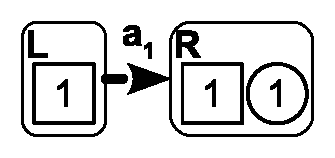
\includegraphics[scale=0.6]{images/process/order/a1}}}
    \caption{Action $a_1$}\label{fig:process:order:a1}
  \end{subfigure}%
  \begin{subfigure}[t]{.2\textwidth}
    \centerline{\fbox{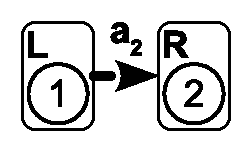
\includegraphics[scale=0.6]{images/process/order/a2}}}
    \caption{Action $a_2$}\label{fig:process:order:a2}
  \end{subfigure}%
  \begin{subfigure}[t]{.3\textwidth}
    \centerline{\fbox{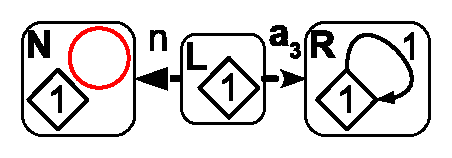
\includegraphics[scale=0.6]{images/process/order/a3}}}
    \caption{Action $a_3$}\label{fig:process:order:a3}
  \end{subfigure}%
  \begin{subfigure}[t]{.2\textwidth}
    \centerline{\fbox{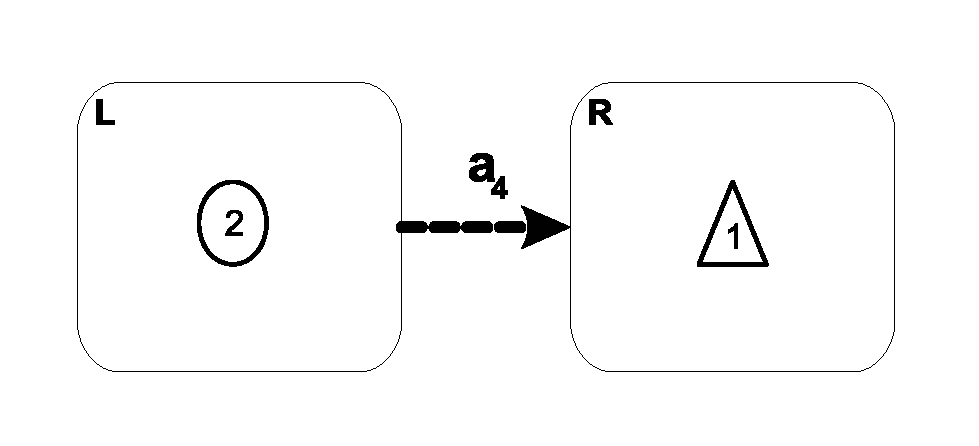
\includegraphics[scale=0.6]{images/process/order/a4}}}
    \caption{Action $a_4$}\label{fig:process:order:a4}
  \end{subfigure}
  \stepcounter{doubly-typed-grammar-counter}
  \caption{Strongly safe grammar GG\arabic{doubly-typed-grammar-counter}}\label{fig:process:order}
\end{figure}

  The causal relation of this grammar is: $a_1 \leq_c a_2, a_2 \leq_c a_4, a_1 \leq_c a_4, a_3 \leq_c a_3$. Without the NACs, any sequentialization where the order $a_1 < a_2 < a_4$ is maintained would be valid, such as $[a_1, a_2, a_3, a_4]$, $[a_1,a_3,a_2,a_4]$, $[a_3, a_1, a_2, a_4]$ and $[a_1,a_2,a_4,a_3]$.

  However, as this grammar have NACs, the following conditional conflicts and dependencies have been identified:
\begin{itemize}
  \item delete-forbids: $a_4 <_{df} a_3$ caused by the deletion of $\Circle_2$.
  \item produce-forbids: $a_3 <_{pf} a_1$ caused by creation of $\Circle_1$, and $a_3 <_{pf} a_2$ caused by the creation of $\Circle_2$.
\end{itemize}

  Notice that, despite of the fact that $a_2$ deletes $\Circle_1$, which triggers the NAC of $a_3$, $a_2 <_{df} a_3$ is not a delete-forbid dependency because $a_2$ also creates $\Circle_2$, an element that still triggers the same NAC. Therefore the transformations when searching for the dependency between $a_2$ to $a_3$ are not valid.

  None of these conflicts or dependencies are \emph{concrete}, they depend on how the actions are applied according to the causal relation to exist. This situation is summarized in Figure~\ref{fig:process:order:cycle}, where the causal relation, the conflicts and dependencies are represented (without the explicit representation of transitivity and reflexivity). At first, if we are to consider all the relations as they are calculated by the diagrams themselves, there would be no possible sequentialization for this actions, denoted by the cycle in the ordering graph.

\begin{figure}[!ht]
  \centering
  \fbox{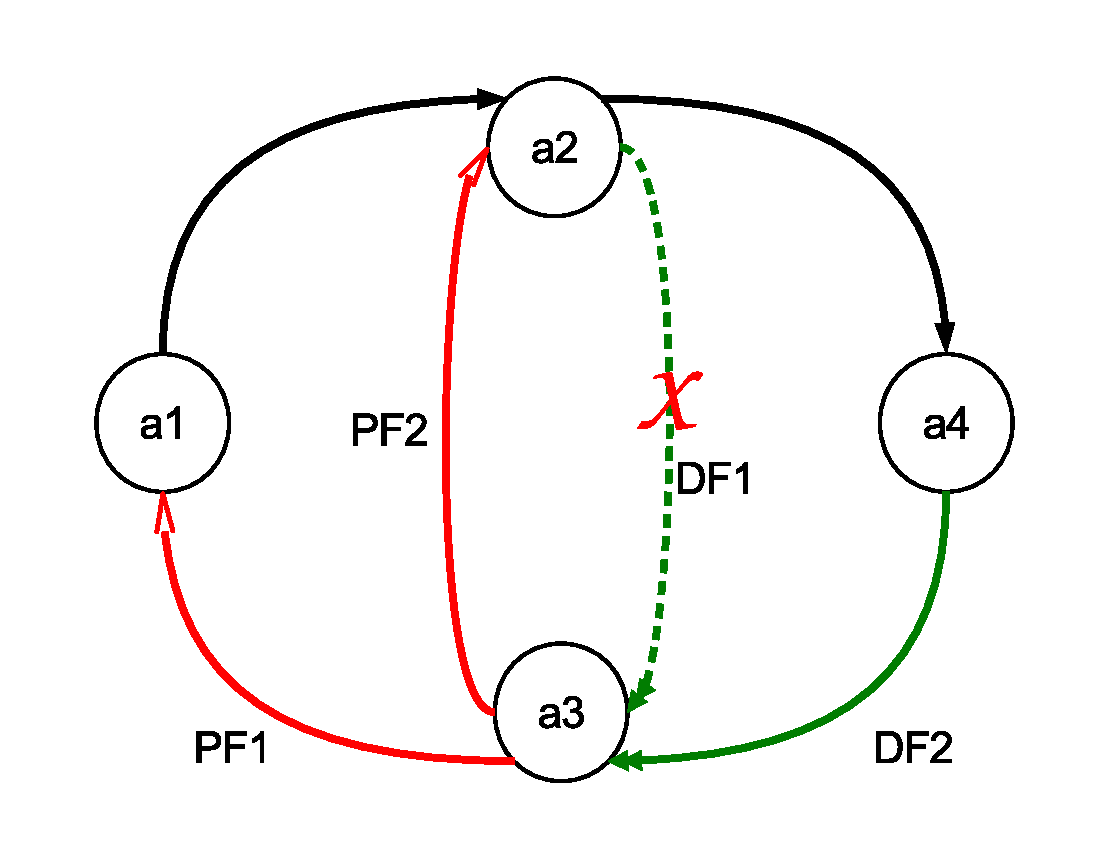
\includegraphics[scale=1]{images/process/order/cycle}}
  \caption{Cycle due to conditional conflicts and dependencies}\label{fig:process:order:cycle}
\end{figure}

  Regarding the element $\Circle_1$, we have an abstract produce-forbid conflict as $a_3$ can be applied before $a_1$ creates it or after $a_2$ deletes it. Thus it is possible to apply $a_3$ as long as it is not applied between $a_1$ and $a_2$. As for the element $\Circle_2$, we have an abstract produce-forbid conflict as $a_3$ can be applied before $a_2$ creates it or after $a_4$ deletes it.

  In fact, we have that the actions of this particular grammar can be executed in any total ordering of its causal relation $a_1 \leq_c a_2, a_2 \leq_c a_4, a_1 \leq_c a_4, a_3 \leq_c a_3$ that also respects the \emph{restrictions} given by the abstract dependency/conflict tuples $(a_3,a_1,a_2)$ and $(a_3,a_2,a_4)$. There exist two such sequentializations, namely: $[a_3, a_1, a_2, a_4]$ and $[a_1,a_2,a_4,a_3]$.
\end{example}

\begin{remark}[Abstract Dependencies and Conflicts] The existence of an abstract produce-forbid conflict, triggered by an element $x$ is always conditioned to the existence of an action which deletes $x$. Given an action $a_1$ which creates $x$, an action $a_2$ whose NAC forbids $x$ and provided a configuration where $a_1$ was applied before $a_2$, we have that $a_2$ can be applied only after an action $a_3$ which deletes $x$ has been applied.
\iffalse
  However, $a_3$ may also cause a new produce-forbid conflict on $a_2$ by creating a new element $y$ which is also forbidden by a NAC of $a_2$, on which case $a_2$ can only be applied if there is another action $a_4$ which ``turns off'' the conflict caused by $a_3$ by deleting $y$.
\fi
  In general, for each abstract produce-forbid conflict $a_2 <_{pf} a_1$ caused by an element $x$, we have that $a_2$ must be successfully applied before $a_1$ or after an action $a_{j}$ where $a_i$ deletes $x$ and $a_i \leq a_j$.

  Analogously, for each abstract delete-forbid dependency $a_1 <_{df} a_2$ caused by an element $x$, we have that $a_2$ must be successfully applied after $a_1$ or before an action $a_j$ where $a_i$ creates $x$ and $a_j \leq a_i$.
\end{remark}

\newadd{There is one last problem that arises with the addition of NACs in Occurrence Graph Grammars. Given a strongly safe graph grammar \doublyTypedGraphGrammarCore{} with NACs, if there is an action $a_i \in P$ which has a NAC triggered by an element $x \in I^{C^T}$, i.e. an element that is already present in the initial graph, then there must be an action $a_j \in P$ which deletes $x$ and a ``mandatory'' concrete delete-forbid dependency $a_j <_{df} a_i$, otherwise $GG$ can not be an Occurrence Graph Grammar given that action $a_i$ would never be applicable in any total ordering of actions.}

Having the conflicts and dependencies classified as described above, we can now use these characterizations to extend the original causal relation in order to work with strongly safe graph grammars with (incremental) NACs. The main idea is that non-existent conflicts and dependencies can be discarded, while the concrete ones must be considered together with the causal relation and the abstract ones impose extra restrictions over the causal and (concrete) produce-forbid and delete-forbid relations.

\begin{definition}[Occurence Relation] Given a strongly safe grammar \doublyTypedGraphGrammarCore{}, let $\leq_{df}$ be the set of all its \emph{concrete} delete-forbids pairs and $\leq_{pf}$ be the set of all its \emph{concrete} produce-forbids pairs. Then, its occurrence relation $\leq_o$ of $(P \cup N(C^T) \cup E(C^T))$ is defined as the transitive and reflexive closure of \mbox{$\leq_{c}$ $\cup$ $\leq_{df}$ $\cup$ $\leq_{pf}$}.
\end{definition}

\begin{definition}[Occurence Relation Restrictions] Given a strongly safe grammar \doublyTypedGraphGrammarCore{}, its \emph{occurrence relation restrictions} are the sets containing all its abstract produce-forbid conflicts and delete-forbid dependencies.
\end{definition}

\begin{definition}[Occurrence Graph Grammars]\label{def:ogg} Let \doublyTypedGraphGrammarCore{} be a strongly safe graph grammar. $GG$ is an \emph{occurrence graph grammar} with NACs iff:

  \begin{enumerate}
    \item its occurrence relation $\leq_{o}$ is a partial order such that, for any \mbox{$n \in N(\coreGraph)$}, \mbox{$e \in E(\coreGraph)$} such that $n = s(e)$ or $n = t(e)$, and for any $p \in P$, we have that:
      \begin{itemize}
        \item if $p \leq_o n$, then $p \leq_o e$
        \item if $n \leq_o p$, then $e \leq_o p$;
      \end{itemize}
    \item Let $Min = \{x \in N(\coreGraph) \cup E(\coreGraph)$ $|$ $\not\exists y \in N(\coreGraph) \cup E(\coreGraph)\bullet y \leq_o x \}$, and $G(Min) = \left(N,E,s,t\right)$ such that $N = Min \cap N(\coreGraph)$, $E = Min \cap E(\coreGraph)$, $s = s_{|E}$, and $t = t_{|E}$; then $\initialGraph = G(Min)$;
    \item $\forall p \in P$, $p$ satisfies the \emph{identification condition};
    \item $\forall x \in N(\coreGraph) \cup E(\coreGraph)$, $x$ is consumed by at most one production in $P$, and it is created by at most one production in $P$.
    \item \newadd{$\forall p_i \in P$ with NAC $n_i$, if the triggering element $x$ of $n_i$ is such that $x \in I^{C^T}$, then there must exist another action $p_j \in P$ which deletes $x$ and $p_j <_{df} p_i$ must be a concrete delete-forbid dependency.}
    \item there is at least one total ordering of the actions $a_1,\ldots,a_n \in P$ that respects the occurrence relation restrictions.
  \end{enumerate}
\end{definition}

As was said in the beginning of this chapter, the idea is that an occurrence graph grammar is a suitable way to describe the semantics of a graph grammar, in the sense that it represents both all possible states and changes of states while also being a graph grammar itself.

Our notion of Occurrence Graph Grammar is a restriction over that of~\cite{Corradini1996}. The first four conditions of our definition correspond to those of the Definition 19 in their work, which assure that it is possible to find a sequence of actions that respects the order of creation and deletion of elements given by the causal relation, while extending it to also respect the order imposed by concrete produce-forbids and delete-forbids of the grammar. In other words, it assures that there is no cycle of conflicts and dependencies that can prevent the application of the grammar.

\newadd{The fifth condition works over a specific triggering of NACs which may not be captured by the delete-forbid and produce-forbid relations, which happens when the triggering element of the NAC of an action already exists in the initial graph. If there is an action whose application may be prevented by the existence of an element in the initial graph, then there must be another action responsible for the deletion of that same element which in turn must always be executed before the action with the triggered NAC.}

The sixth condition deals with the conflicts and dependencies induced by NACs that do not participate in the concrete relations, thus generating \emph{intervals} of actions inside of which specific actions can not be applied. If it is possible to find a total ordering of actions regarding the occurrence relation which also obeys the set of restrictions, then it is possible to execute the underlying single typed grammar.

\begin{definition}[Derivation of an Occurrence Graph Grammar with NACs] Given an \occurrenceGrammar{} and a total order $s = a_1,a_2,\ldots,a_n$ of all actions in $A$ which respects the occurrence relation $\leq_o$ and the occurrence relation restrictions of $OGG$, the derivation of $OGG$ regarding $s$ is given by the diagram below, where each individual transformation $t_i : H_{i-1} \xRightarrow{a_i, pre_{a_i}} H_i$ is concrete over the elements of the core graph, as in Definition~\ref{def:strongly-safe-grammar}.


\diagram{
  L_1\ar[d]_{pre_{a_1}} & K_1\ar[d]\ar[l]\ar[r] & R_1\ar[dr]|{post_{a_1}} & & \ldots\ar[dl]|{pre_{a_2}}\ar[dr]|{post_{a_{n-1}}} & & L_n\ar[dl]|{pre_{a_n}} & K_n\ar[d]\ar[l]\ar[r] & R_n\ar[d]^{post_{a_n}} \\
  I^{C^T} & D_1\ar[l]\ar[rr] & & H_1  &  \ldots\ar[l]\ar[r]    & H_{n-1} &    & D_{n}\ar[ll]\ar[r]   & F^{C^T}
}\hfill\\

A derivation for an $OGG$ starts at the initial graph $I^{C^T}$ and terminates at the final graph $F^{C^T}$ of $OGG$, and every intermediary graph is a subgraph of the core graph, i.e. $D_i\xhookrightarrow{} C^T$, $H_i\xhookrightarrow{} C^T$.

\end{definition}

\begin{thm} Given a graph grammar $GG = (T,I^T,P)$ and an Occurrence Graph Grammar with NACs \occurrenceGrammar{}. If we have that:
\begin{itemize}
  \item $\forall a \in A \Rightarrow a \in P$
  \item $I^{C^T} \equiv I^T$
\end{itemize}

Then any derivation represented by $OGG$ is a derivation of $GG$.

\end{thm}

\begin{proof}
  Given a Graph Grammar $GG = (T,I^T,P)$ and an Occurrence Graph Grammar \occurrenceGrammar{} built from $GG$. It is possible to construct a valid derivation of $OGG$ for any total ordering of $A$ which satisfies the occurrence relation and the occurrence relation restrictions of $OGG$.

  Let \mbox{$d = I^{C^T} \xRightarrow{a_1, pre_1} H_1^{C^T} \xRightarrow{a_2, pre_2} H_2^{C^T} \ldots H_{n-1}^{C^T} \xRightarrow{a_n, pre_n} F^{C^T}$} be one of the possible derivations of $OGG$.
  Given the type morphism $t: C \rightarrow T$ of the core graph and the type morphism $dt_i : H_i \rightarrow C^T$ of a $C^T$-double typed graph, it is possible to compose them in a (simple) type morphism $t \circ dt_i : H_i \rightarrow T$. 
  Using the resulting family of (simple) type morphisms obtained by such composition, it is possible to create a diagram \mbox{$d' = I^T \xRightarrow{p_1, m_1} H_1^T \xRightarrow{p_2,m_2} H_2^T \ldots H_{n-1}^T \xRightarrow{p_n, m_n} H_n^T$} which has the format of a derivation of $GG$.

  If the graph grammar $GG$ does not have NACs, the underlying occurrence graph grammar $OGG$ also does not have NACs, and it holds true that $d'$ is a derivation of $GG$, since it was constructed as given by the original definition of occurrence graph grammars in~\cite{Corradini1996}.

  Thus, we need to show that with the addition of (incremental) NACs in $GG$, our extension for the construction of occurrence graph grammars with NACs still guarantees that the derivation $d'$ obtained from $d$ is a valid derivation of $GG$.

  Let $p_i = L^T_i \leftarrow K^T_i \rightarrow R^T_i \in P$ be a rule with an incremental NAC $n_i : L_i^T \rightarrow N_i^T$ which participates in the (candidate) derivation $d'$.
  Assume that $n_i$ is triggered by an elementi $x$ around the match $m_i : L_i^T \rightarrow H^T_{i-1}$ in the derivation. There are four possible cases that could lead to this configuration:
\begin{enumerate}
  \item $x \in I^T$ and there is no rule which deletes it.
  \item $x \in I^T$, but the rule $p_k$ which deletes it was applied after $p_i$, i.e. $p_i < p_k$. 
  \item $x$ was created by a rule $p_j$ applied before $p_i$ and there is no other rule which deletes $x$, i.e $p_j < p_i$.
  \item $x$ was created by a rule $p_j$ applied before $p_i$ and the rule $p_k$ which deletes $x$ was applied after $p_i$, i.e. $p_j < p_i < p_k$.
\end{enumerate}

  The construction of the occurrence graph grammar would identify these problems as listed below:

  \newadd{In the first case, the condition which requires the existence of another action $p_j$ responsible for the deletion of $x$ with a concrete delete-forbid dependency $p_j <_{df} p_i$ between them would be violated, therefore $OGG$ would not be a valid Occurrence Graph Grammar.}

  In the second case, there would be a concrete delete-forbid dependency between actions $a_k <_{df} a_i$, therefore this dependency would be present on the occurrence relation and any total ordering where $a_i < a_k$ would not satisfy the $OGG$ constraints.

  In the third case, there would be a concrete produce-forbid conflict between actions $a_i <_{pf} a_j$, this conflict would thus be present on the occurrence relation and any total ordering where $a_j < a_k$ would not satisfy the $OGG$ constraints.

  In the fourth case, there would be an abstract delete-forbid dependency and/or an abstract produce-forbid conflict denoted by the tuple $(a_i,a_j,a_k)$, which would be included in the set of occurrence relation restrictions and forbid any total ordering of actions where $a_j < a_i < a_k$.

  Therefore, given that either of the situations described above would result in a total ordering of actions in $A$ which do not satisfy the constraints of an Occurrence Graph Grammar with NACs \occurrenceGrammar{}, $d'$ not being a derivation of $GG$ would contradict the fact the $d$ is a derivation of $OGG$, because it would be based on a total ordering which do not satisfy the constraints of its underlying Occurrence Graph Grammar.

  %\newadd{Para o 3.34 tens que arrgumentar que , para qualquer ordem total que satisfaça a OGG com NACs, cada acão  de P que envolve uma NAC pode ser executada depois das ações que vem antes dela na ordem, e isto seria garantido pelas restricoes que tu impuseste ao gerar a OGG.}
\end{proof}


\begin{thm} Given a Graph Grammar with NACs ${GG = (T,I^T,P)}$, any derivation of $GG$ generates an Occurrence Graph Grammar with NACs \occurrenceGrammar{}. 
\end{thm}

\begin{proof}

Let $d = I^T \xRightarrow{p_1, m_1} H_1 \xRightarrow{p_2, m_2} H_2 \ldots H_{n-1} \xRightarrow{p_n, m_n} H_n$ be a valid derivation of $GG$.
We have that $d$ provides a total order of rules $p_i \in P$ in which it is possible to apply a particular number of rules. 
Therefore, if we calculate the colimit of the diagram defined by derivation $d$ the result is a graph $C^T$ containing all the elements ever used in that derivation.
This colimit also identifies the common elements among the rules and initial (and final) graph. Thus, the colimit object $C^T$ is also a core graph.

Given the rules $p_1, p_2,\ldots,p_n$ used in the derivation, if we consider their morphisms to $C^T$ as typing morphisms, we arive at a set of double-typed graph rules $A = (a_1,a_2,\ldots,a_n)$ over $C^T$.
Similarly, if we consider the morphism from the initial graph $I^T$ to the colimit as a typing morphism, we arive at a double-typed graph $I^{C^T}$.
Thus, the grammar defined by $OGG = (C^T,I^{C^T},A)$ is in fact a strongly safe graph grammar, therefore a candidate to be an occurrence graph grammar with NACs.

We now have to prove that (1) the occurrence relation $\leq_o$ underlying $OGG$ is a partial order and that (2) there is at least one total ordering of $\leq_o$ which also respects the occurrence relation restrictions generated by the analysis of conflicts and dependencies induced by NACs in $OGG$.

If we use the the same order of actions in $A$ given by the application of their correspondent graph rules from $P$ in the derivation $d$, we have a total order $<_o$ which allows the application of all actions in $A$, thus $\leq_o$ must be a partial order.

  As for the occurrence relation restrictions, we have at least one total order which satisfies them, also given the same order of rules application in $d$.
  If this order did not satisfy these restrictions, then there would be at least one triggered NAC disabling a transformation in $d$, therefore $d$ would not be a valid derivation.

\end{proof}

\begin{definition}[Semantics of a Graph Grammar] Given a Graph Grammar \graphGrammar{} the semantics of $GG$ is described by the set of $OGGs$ corresponding to its derivations.
\end{definition}
